\documentclass[fleqn, a4paper]{article}

\usepackage{a4wide}
%\setlength{\parindent}{0pt}
%\setlength{\parskip}{6pt plus 2pt minus 1pt}
%\usepackage{lscape}

\usepackage[utf8]{inputenc}

\usepackage[round,longnamesfirst]{natbib}
\usepackage{graphicx,keyval,thumbpdf,url}
\usepackage{hyperref}

\usepackage{amsmath}
\usepackage{amsfonts}


\usepackage{Sweave}

\AtBeginDocument{\setkeys{Gin}{width=0.6\textwidth}}

\newcommand{\strong}[1]{{\normalfont\fontseries{b}\selectfont #1}}
\newcommand{\class}[1]{\mbox{\textsf{#1}}}
\newcommand{\func}[1]{\mbox{\texttt{#1()}}}
\newcommand{\code}[1]{\mbox{\texttt{#1}}}
\newcommand{\pkg}[1]{\strong{#1}}
\newcommand{\samp}[1]{`\mbox{\texttt{#1}}'}
\newcommand{\proglang}[1]{\textsf{#1}}
\newcommand{\set}[1]{\mathcal{#1}}
\newcommand{\sQuote}[1]{`{#1}'}
\newcommand{\dQuote}[1]{``{#1}''}
\newcommand\R{{\mathbb{R}}}

\DeclareMathOperator*{\argmin}{argmin}
\DeclareMathOperator*{\argmax}{argmax}

\hyphenation{Brusco}

%% \VignetteIndexEntry{Introduction to seriation}



\begin{document}



\title{Getting Things in Order: An introduction to the 
R~package~\pkg{seriation}}
\author{Michael Hahsler, Kurt Hornik and Christian Buchta}
\maketitle
\sloppy

\abstract{Seriation, i.e., finding a linear order for a set of objects
  given data and a loss or merit function, is a basic problem in data
  analysis.  Caused by the problem's combinatorial nature, it is hard to
  solve for all but very small sets.  Nevertheless, both exact solution
  methods and heuristics are available.  In this paper we present the
  package~\pkg{seriation} which provides the infrastructure for
  seriation with R.  The infrastructure comprises data structures to
  represent linear orders as permutation vectors, a wide array of
  seriation methods using a consistent interface, a method to calculate
  the value of various loss and merit functions, and several
  visualization techniques which build on seriation. To illustrate how
  easily the package can be applied for a variety of applications, a
  comprehensive collection of examples is presented.}

\section{Introduction}

A basic problem in data analysis, called \emph{seriation} or sometimes
\emph{sequencing}, is to arrange all objects in a set in a linear order
given available data and some loss or merit function in order to
reveal structural information.  Together with
cluster analysis and variable selection, seriation is an important
problem in the field of \emph{combinatorial data
  analysis}~\citep{seriation:Arabie:1996}.  Solving problems in
combinatorial data analysis requires the solution of discrete
optimization problems which, in the most general case, involves
evaluating all feasible solutions.  Due to the combinatorial nature, the
number of possible solutions grows with problem size (number of objects)
by the order $O(n!)$.  This makes a brute-force enumerative approach
infeasible for all but very small problems.  To solve larger problems
(with up to 40 objects), partial enumeration methods can be used.  For
example, \cite{seriation:Hubert:1987} propose dynamic programming and
\cite{seriation:Brusco:2005} use a branch-and-bound strategy.  For even
larger problems only heuristics can be employed.

It has to be noted that seriation has a rich history in archeology.
\cite{seriation:Petrie:1899} was the first to use seriation as a formal method.
He applied it to find a chronological order for graves discovered in the Nile
area given objects found there. He used a cross-tabulation of grave sites and
objects and rearranged the table using row and column permutations till all
large values were close to the diagonal. In the rearranged table graves with
similar objects are closer to each other. Together with the assumption that
different objects continuously come into and go out of fashion, the order of
graves in the rearranged table suggests a chronological order.
Initially, the rearrangement of rows and columns of this
contingency table was done manually and the adequacy was only judged
subjectively by the researcher.  Later, \cite{seriation:Robinson:1951},
\cite{seriation:Kendall:1971} and others proposed measures of agreement
between rows to quantify optimality of the resulting table.  A
comprehensive description of the development of seriation in archeology
is presented by \cite{seriation:Ihm:2005}.

Techniques related to seriation are also popular in several other
fields.  Especially in ecology scaling techniques are used under the
name \emph{ordination}.  For these applications several R packages
already exist (e.g., \pkg{ade4}~\citep{seriation:Chessel:2007} and
\pkg{vegan}~\citep{seriation:Oksanen:2007}). This paper describes the new
package \pkg{seriation} which differs from existing packages in the
following ways:
\begin{enumerate}
 \item \pkg{seriation} provides a flexible infrastructure for seriation;
 \item \pkg{seriation} focuses on seriation as a combinatorial
  optimization problem.
\end{enumerate}

This paper starts with a formal introduction of the seriation problem as
a combinatorial optimization problem in Section~\ref{sec:seriation}.  In
Section~\ref{sec:methods} we give an overview of seriation methods.  In
Section~\ref{sec:infrastructure} we present the infrastructure provided
by the package~\pkg{seriation}.  Several examples and applications for
seriation are given in Section~\ref{sec:example}.  We conclude with
Section~\ref{sec:conclusion}.

\section{Seriation as a combinatorial optimization problem}
\label{sec:seriation}

To seriate a set of $n$ objects $\{O_1,\dots,O_n\}$ one typically starts with an
$n \times n$ symmetric dissimilarity matrix~$\mathbf{D} = (d_{ij})$ where
$d_{ij}$ for $1 \le i,j \le n$ represents the dissimilarity between the objects
$O_i$ and $O_j$ and all $d_{ii} = 0$.  We define a permutation function $\Psi$
as a function which reorders the objects in $\mathbf{D}$ by simultaneously
permuting rows and columns.  The seriation problem is to find a permutation
function $\Psi$
%$\{1,\dots,n\} \rightarrow \{1,\dots,n\}$, i.e. a
%bijection that maps the set of indices of the objects (and equally of rows and
%columns of $\mathbf{D}$) onto itself, 
which optimizes the value of a given loss function $L$ or merit function $M$.
This results in the optimization problems
\begin{equation}
    L(\Psi(\mathbf{D})) \rightarrow \mathrm{min}_\Psi \quad \text{or} \quad
    M(\Psi(\mathbf{D})) \rightarrow \mathrm{max}_\Psi\text{,}
\end{equation}
respectively.
%This is clearly a hard discrete optimization problem since the number of 
%possible permutations is $n!$ which makes an exhaustive 
%search for sets with a medium to large number of objects infeasible.
%Partial enumeration methods and heuristics can be used. Such methods are 
%presented in Section~\ref{sec:methods}.
%But first, we review commonly used loss functions in the following section.
%\marginpar{two-mode data missing}

A symmetric dissimilarity matrix is known as \emph{two-way one-mode}
data since it has columns and rows (two-way) but only represents one set
of objects (one-mode).  Seriation is also possible for two-way two-mode
data which are represented by a general positive matrix.  In such data
columns and rows represent two sets of objects which are reordered
simultaneously.  For loss functions for two-way two-mode data the
optimal order of columns can be dependent of the order of rows and vice
versa or it can be independent allowing for breaking the optimization
down into two separate problems, one for the columns and one for the
rows.  Another way to deal with the seriation for two-way two-mode data
is to calculate two dissimilarity matrices, one for each mode, and then
solve two seriation problem on two-way one-mode data.  Furthermore,
seriation can be generalized to $k$-way $k$-mode data in the form of a
$k$-dimensional array by defining suitable loss functions for such data
or by breaking the problem down into several lower dimensional
independent problems which can be solved.


In the following subsections, we review some commonly used loss
functions.  Most functions are used for two-way one-mode data but the
measure of effectiveness and stress can be also used for two-way
two-mode data.


%\section{Loss functions}
%\label{sec:criteria}
%In the literature several loss functions are suggested.
%We review the most commonly used functions.

\subsection{Column/row gradient measures}

A symmetric dissimilarity matrix 
where the values in all rows and columns only increase when
moving away from the main diagonal is called a perfect 
\emph{anti-Robinson matrix} after the
statistician \cite{seriation:Robinson:1951}. Formally, 
an $n \times n$ dissimilarity matrix $\mathbf{D}$ is in anti-Robinson form if, 
and only if the following two gradient conditions 
hold~\citep{seriation:Hubert:1987}:
\begin{align}
    \text{within rows:} & \quad  d_{ik} \le d_{ij} \quad \text{for} 
        \quad 1 \le i < k < j \le n; \\ 
    \text{within columns:} & \quad  d_{kj} \le d_{ij} \quad \text{for} 
        \quad 1 \le i < k < j \le n.
\end{align}

In an anti-Robinson matrix the smallest dissimilarity values appear
close to the main diagonal, therefore, the closer objects are together
in the order of the matrix, the higher their similarity.  This provides
a natural objective for seriation.

It has to be noted that $\mathbf{D}$ can be brought into a perfect
anti-Robinson form by row and column permutation whenever $\mathbf{D}$  is an
ultrametric or $\mathbf{D}$ has an exact Euclidean representation in a single
dimension~\citep{seriation:Hubert:1987}. However, for most data only an
approximation to the anti-Robinson form is possible.

A suitable merit measure which quantifies the divergence of a matrix from the
anti-Robinson form was given by \cite{seriation:Hubert:1987} as
\begin{equation}
    M(\mathbf{D}) = 
    \sum_{i<k<j}f(d_{ik}, d_{ij}) + \sum_{i<k<j}f(d_{kj}, d_{ij}) 
    \label{equ:gradient}
\end{equation}
where $f(\cdot,\cdot)$ is a function which defines how a violation or
satisfaction of a gradient condition for an object triple ($O_i$, $O_k$ and
$O_j$) is counted.  \cite{seriation:Hubert:1987} suggest two functions. The
first function is given by:
\begin{equation}
    f(z,y) = \mathrm{sign}(y-z) = 
    \begin{cases}
        +1 \quad \text{if} \quad z < y; \\
        \phantom{+}0 \quad \text{if} \quad z = y; \\
        -1 \quad \text{if} \quad z > y.
    \end{cases}
\end{equation}
It results in the raw number of triples satisfying the gradient
constraints minus triples which violate the constraints. 

The second function is defined as:
\begin{equation}
    f(z,y) = |y-z|\mathrm{sign}(y-z) = y-z
\end{equation}
It weighs each satisfaction or violation by its
magnitude given by the absolute difference between the values.

\subsection{Anti-Robinson events}
An even simpler loss function can be created in the same way as the gradient
measures above by concentrating on violations only. 
\begin{equation}
    L(\mathbf{D}) = 
    \sum_{i<k<j}f(d_{ik}, d_{ij}) + \sum_{i<k<j}f(d_{kj}, d_{ij}) 
\end{equation}

To only count the violations we use
\begin{equation}
    f(z, y) = I(z, y) = 
    \begin{cases}
        1 \quad \text{if} \quad z < y \quad \text{and} \\
        0 \quad \text{otherwise.}
    \end{cases}
\end{equation}
$I(\cdot)$ is an indicator function returning $1$ only for violations.
\cite{seriation:Chen:2002} presented a formulation for an equivalent 
loss function and called the violations \emph{anti-Robinson events}.
\cite{seriation:Chen:2002} also introduced a weighted versions of the loss 
function resulting in
\begin{equation}
    f(z, y) = |y-z|I(z, y)
\end{equation}
using the absolute deviations as weights.

\subsection{Hamiltonian path length}
The dissimilarity matrix $\mathbf{D}$ can be represented as a finite weighted
graph $G = (\Omega,E)$ where the set of objects $\Omega$ constitute the
vertices and each edge $e_{ij} \in E$ between the objects $O_i, O_j \in \Omega$ 
has a weight $w_{ij}$ associated which represents the dissimilarity $d_{ij}$.

Such a graph can be used for seriation~\citep[see,
e.g.,][]{seriation:Hubert:1974,seriation:Caraux:2005}.  An order $\Psi$
of the objects can be seen as a path through the graph where each node
is visited exactly once, i.e., a Hamiltonian path.  Minimizing the
Hamiltonian path length results in a seriation optimal with respect to
dissimilarities between neighboring objects.  The loss function based on
the Hamiltonian path length is:
\begin{equation}
    L(\mathbf{D}) = \sum_{i=1}^{n-1} d_{i,i+1}.
\end{equation}

Note that the length of the Hamiltonian path is equal to the value of the
\emph{minimal span loss function} \citep[as used by][]{seriation:Chen:2002},
and both notions are related to the \emph{traveling salesperson
problem}~\citep{seriation:Gutin:2002}.

\subsection{Inertia criterion} 
Another way to look at the seriation problem is not to focus on placing small
dissimilarity values close to the diagonal, but to push large values away from
it. A function to quantify this is the moment of inertia of dissimilarity
values around the diagonal \citep{seriation:Caraux:2005} defined as
\begin{equation}
    M(\mathbf{D}) = \sum_{i=1}^n \sum_{j=1}^n d_{ij}|i-j|^2.
\end{equation}
$|i-j|^2$ is used as a measure for the distance to the diagonal and $d_{ij}$
gives the weight.  This is a merit function since the sum increases when higher
dissimilarity values are placed farther away from the diagonal.

\subsection{Least squares criterion} 
Another natural loss function for seriation is to quantify the deviations
between the dissimilarities in $\mathbf{D}$ and the rank differences of the
objects.  Such deviations can be measured, e.g, by the sum of squares of
deviations \citep{seriation:Caraux:2005} defined by
\begin{equation}
    L(\mathbf{D}) = \sum_{i=1}^n \sum_{j=1}^n (d_{ij} - |i-j|)^2,
\end{equation}
where $|i-j|$ is the rank difference or gap between $O_i$ and $O_j$.

The least squares criterion defined here is related to uni-dimensional
scaling~\citep{seriation:Leeuw:2005}, where the objective is to place all
objects on a straight line such that the dissimilarities in $\mathbf{D}$ are
preserved by the relative positions in the best possible way.  The optimization
problem of uni-dimensional scaling is to minimize $\sum_{i=1}^n \sum_{j=1}^n
(d_{ij} - |x_i-x_j|)^2$ which is close to the seriation problem, but in
addition to the ranking of the objects also takes the distances between objects
on the resulting scale into account.

Note that if Euclidean distance is used to calculate $\mathbf{D}$ from a data
matrix $\mathbf{X}$, the order of the elements in $\mathbf{X}$ by projecting
them on the first principal component of $\mathbf{X}$ minimizes 
the loss function of uni-dimensional scaling (using squared distances) and
also provides good solutions for this seriation criterion.

\subsection{Measure of effectiveness}
\label{sec:ME}

\cite{seriation:McCormick:1972} defined the
\emph{measure of effectiveness (ME)} for an $n \times m$ matrix $\mathbf{X} =
(x_{ij})$ as
\begin{equation}
    M(\mathbf{X}) =
    \frac{1}{2}
    \sum_{i=1}^{n} \sum_{j=1}^{m} x_{ij}[x_{i,j+1}+x_{i,j-1}+
        x_{i+1,j}+x_{i-1,j}]
    \label{equ:ME}
\end{equation}
with, by convention $x_{0,j}=x_{n+1,j}=x_{i,0}=x_{i,m+1}=0$.  ME is maximized
if each element is as closely related numerically to its four neighboring
elements as possible.

ME was developed for two-way two-mode data, however, ME can also be used for a
symmetric  matrix (one-mode data) and gets maximal only if all large values are
grouped together around the main diagonal. 

Note that the definition in equation~(\ref{equ:ME}) 
can be rewritten as
\begin{equation}
    M(\mathbf{X}) =
    \frac{1}{2}
    \sum_{i=1}^{n} \sum_{j=1}^{m} x_{ij}[x_{i,j+1}+x_{i,j-1}] +
    \sum_{i=1}^{n} \sum_{j=1}^{m} x_{ij}[x_{i+1,j}+x_{i-1,j}]
\end{equation}
showing that the contribution of column and row order to the loss function is
additive and thus the permutation of columns and rows are independent. 

\subsection{Stress}
\label{sec:stress}

Stress measures the conciseness of the presentation of a matrix
(two-mode data) and can be seen as a purity function which compares the
values in a matrix with their neighbors.  The stress measures used here
are computed as the sum of squared distances of each matrix entry from
its adjacent entries.  \cite{seriation:Niermann:2005} defined for an $n
\times m$ matrix $\mathbf{X} = (x_{ij})$ two types of neighborhoods:

\begin{itemize}
    \item The Moore neighborhood comprises the (at most) eight adjacent entries.
        The local stress measure for element $x_{ij}$ is defined as
        \begin{equation}
            \sigma_{ij} = \sum_{k=\max(1,i-1)}^{\min(n,i+1)} 
                \sum_{l=\max(1,j-1)}^{\min(m,j+1)} 
                (x_{ij} - x_{kl})^2
        \end{equation}

    \item The Neumann neighborhood comprises the (at most) four adjacent entries
        resulting in the local stress of $x_{ij}$ of
        \begin{equation}
            \sigma_{ij} = 
            \sum_{k=\max(1,i-1)}^{\min(n,i+1)} (x_{ij} - x_{kj})^2 + 
            \sum_{l=\max(1,j-1)}^{\min(m,j+1)} (x_{ij} - x_{il})^2
            %(x_{ij} - x(i-1,j))^2 + (x_{ij} - x(i+1,j))^2 +
            %(x_{ij} - x(i,j-1))^2 + (x_{ij} - x(i,j+1))^2
        \end{equation}
\end{itemize}

Both local stress measures can be used to construct a global measure for the
whole matrix by summing over all entries which can be used as a loss function:
\begin{equation}
    L(\mathbf{X}) = 
    \sum_{i=1}^n \sum_{j=1}^m \sigma_{ij}
\end{equation}

The major difference between the Moore and the Neumann neighborhood is that for
the later the contribution of row and column permutations to stress are
independent and thus can be optimized independently. 

Stress can be also used as a loss function for
symmetric proximity matrices (one-mode data).
%, 
%since it can only be optimal, if large values are
%concentrated around the main diagonal. 
Note also, that stress with Neumann
neighborhood is related to the measure of effectiveness defined above (in
Section~\ref{sec:ME}) since both measures are optimal if for each cell the cell
and its four neighbors are numerically as similar as possible.

\section{Seriation methods}
\label{sec:methods}

Solving the discrete optimization problem for seriation with most loss/merit
functions is clearly very hard. The number of possible permutations is $n!$
which makes an exhaustive search for sets with a medium to large number of
objects infeasible.  In this section, we describe some methods (partial
enumeration, heuristics and other methods) which are typically used for
seriation. For each method we state for which type of loss/merit functions it
is suitable and if it finds the optimum or is a heuristic.

\subsection{Partial enumeration methods}

Partial enumeration methods search for the exact solution of a
combinatorial optimization problem.  Exploiting properties of the search
space, only a subset of the enormous number of possible combinations has
to be evaluated.  Popular partial enumeration methods which are used for
seriation are \emph{dynamic programming}~\citep{seriation:Hubert:1987}
and \emph{branch-and-bound}~\citep{seriation:Brusco:2005}.

Dynamic programming recursively searches for the optimal solution checking and
storing $2^n-1$ results. Although $2^n-1$ grows at a lower rate than $n!$ and
is for $n \gg 3$ considerably smaller, the storage requirements of $2^n-1$
results still grow fast, limiting the maximal problem size severely. For
example, for $n=30$ more than one billion results have to be calculated and
stored, clearly a number too large for the main memory capacity of most current
computers.

Branch-and-bound has only very moderate storage requirements. The
forward-branching procedure~\citep{seriation:Brusco:2005} starts to build
partial permutations from left (first position) to right. At each step, it is
checked if the permutation is valid and several fathoming tests are performed
to check if the algorithm should continue with the partial permutation.  The
most important fathoming test is the boundary test, which checks if the partial
permutation can possibly lead to a complete permutation with a better solution
than the currently best one.  In this way large parts of the search space can
be omitted. However, in contrast to the dynamic programming approach, the
reduction of search space is strongly data dependent and poorly structured
data can lead to very poor performance.  With branch-and-bound slightly larger
problems can be solved than with dynamic programming in reasonable time.
\cite{seriation:Brusco:2005} state that depending on the data, in some cases
proximity matrices with 40 or more objects can be handled with current 
hardware.

Partial enumeration methods can be used to find the exact solution
independently of the loss/merit function. However, partial enumeration is
limited to only relatively small problems.

\subsection{Traveling salesperson problem solver}

Seriation by minimizing the length of a Hamiltonian path through a graph
is equal to solving a traveling salesperson problem.  The traveling
salesperson or salesman problem (TSP) is a well known and well
researched combinatorial optimization problem. The goal is to find the
shortest tour that visits each city in a given list exactly once and
then returns to the starting city. In graph theory a TSP tour is called
a \emph{Hamiltonian cycle.} But for the seriation problem, we are
looking for a Hamiltonian path. \cite{seriation:Garfinkel:1985}
described a simple transformation of the TSP to find the shortest
Hamiltonian path.  An additional row and column of 0's is added
(sometimes this is referred to as a \emph{dummy city}) to the original
$n \times n$ dissimilarity matrix $\mathbf{D}$.  The solution of this
$(n+1)$-city TSP, gives the shortest path where the city representing
the added row/column cuts the cycle into a linear path.

As the general seriation problem, solving the TSP is difficult.  In the
seriation case with $n+1$ cities, $n!$ tours have to be checked. However,
despite this vast searching space, small instances can be solved efficiently
using dynamic programming \citep{seriation:Held:1962} and larger instances of
several hundred objects can be solved using \emph{branch-and-cut}
algorithms~\citep{seriation:Padberg:1990}. For even larger instances or if
running time is critical, a wide array of heuristics are available, ranging
from simple nearest neighbor approaches to construct a
tour~\citep{seriation:Rosenkrantz:1977} to complex heuristics like the
Lin-Kernighan heuristic~\citep{seriation:Lin:1973}.  A comprehensive overview
of heuristics and exact methods can be found in \cite{seriation:Gutin:2002}.


\subsection{Bond energy algorithm}

The \emph{bond energy algorithm}~\citep[BEA;][]{seriation:McCormick:1972} is a
simple heuristic to rearrange columns and rows of a matrix such that each entry
is as closely numerically related to its four neighbors as possible.  To
achieve this, BEA tries to maximize the measure of effectiveness (ME) defined
in Section~\ref{sec:ME}.  For optimizing the ME, columns and rows can be
treated separately since changing the order of rows does not influence the ME
contributions of the columns and vice versa. BEA consists of the
following three steps:
\begin{enumerate}
 \item Place one randomly chosen column.  
 \item Try to place each remaining column at each possible position
  left, right and between the already placed columns and calculate every
  time the increase in ME.  Choose the column and position which gives
  the largest increase in ME and place the column.  Repeat till all
  columns are placed.
 \item Repeat procedure with rows.
\end{enumerate}

This greedy algorithm works fast and is only dependent on the choice of the
first column/row. This dependence can be reduced by repeating the
procedure several times with different choices and returning the solution
with the highest ME.

Although \cite{seriation:McCormick:1972} use BEA also for non-binary data,
\cite{seriation:Arabie:1990} argue that the measure of effectiveness only
serves its indended purpose of finding a arrangement which is
close to Robinson form for binary data and should therefore only be
used for binary data.

\cite{seriation:Lenstra:1974} notes that the optimization problem of BEA
can be stated as two independent traveling salesperson problems (TSPs).
For example, the row TSP for an $n \times m$ matrix~$\mathbf{X}$
consists of $n$ cities with an $n \times n$ distance matrix~$\mathbf{D}$
where the distances are
\begin{displaymath}
    d_{ij} = -\sum_{k=1}^m x_{ik}x_{jk}.
\end{displaymath}
BEA is in fact a simple suboptimal TSP heuristic using this distances
and instead of BEA any TSP solver can be used to obtain an order.
With an exact TSP solver, the optimal solution can be found.

\subsection{Hierarchical clustering}
\label{sec:hierarchical_clustering}

Hierarchical clustering produces a series of nested clusterings which
can be visualized by a dendrogram, a tree where each internal node
represents a split into subtrees and has a measure of
similarity/dissimilarity attached to it.  As a simple heuristic to find
a linear order of objects, the order of the leaf nodes in a dendrogram
structure can be used. This idea is used, e.g., by heat maps to reorder
rows and columns with the aim to place more similar objects and
variables closer together.

%For hierarchical clustering several methods are available (e.g.,
%single linkage, average linkage, complete linkage, ward method) resulting in
%different dendrograms. 
%However, 
The order of leaf nodes in a dendrogram is not unique.  A binary
(two-way splits only) dendrogram for $n$ objects has $2^{n-1}$ internal
nodes and at each internal node the left and right subtree (or leaves)
can be swapped resulting in $2^{n-1}$ distinct leaf orderings.  To find
an unique or optimal order, an additional criterion has to be defined.
\cite{seriation:Gruvaeus:1972} suggest to obtain a unique order by
requiring to order the leaf nodes such that at each level the objects at
the edge of each cluster are adjacent to that object outside the cluster
to which it is nearest.

\cite{seriation:Bar-Joseph:2001} suggest to rearrange the dendrogram such that
the Hamiltonian path connecting the leaves is minimized and called this the
optimal leaf order. The authors also present a fast algorithm with time
complexity $O(n^4)$ to solve this optimization problem. Note that this problem
is related to the TSP described above, however, the given dendrogram structure
significantly reduces the number of permissible permutations making the problem
easier.

Although hierarchical clustering solves an optimization problem different to
the seriation problem discussed in this paper, hierarchical clustering still
can produce useful orderings, e.g., for visualization.

\subsection{Rank-two ellipse seriation}

\cite{seriation:Chen:2002} proposes to
generate a sequence of correlation matrices
$R^1, R^2, \ldots$. $R^1$ is the correlation matrix
of the original distance matrix $\mathbf{D}$ and
\begin{equation}
R^{n+1} = \phi R^n,
\end{equation}
where $\phi(\cdot)$ calculates a correlation matrix.

The rank of the matrix $R^n$ falls with increasing $n$. The sequence
is continued till the first matrix in the sequence has a rank of 2.
Projecting all points in this matrix on the first two eigenvectors,
all points fall on an ellipse. The order of the points on this ellipse
is the resulting order where the ellipse can be cut at any of the 
two interception points (top or bottom) with the vertical axis.

Although the rank-two ellipse seriation procedure does not try to solve a
combinatorial optimization problem, it still provides for some cases a useful
ordering.

\section{The package infrastructure}
\label{sec:infrastructure}

The \pkg{seriation} package provides the data structures and some algorithms
to efficiently handle seriation with R. As the input data for seriation R 
already provides

\begin{itemize}
    \item for two-way one-mode data the class \code{dist},
    \item for two-way two-mode data the class \code{matrix}, and
    \item for $k$-way $k$-mode data the class \code{array}.
\end{itemize}


\begin{figure}[tp]
    \centerline{
    %\includegraphics[width=12cm]{infrastructure}}
    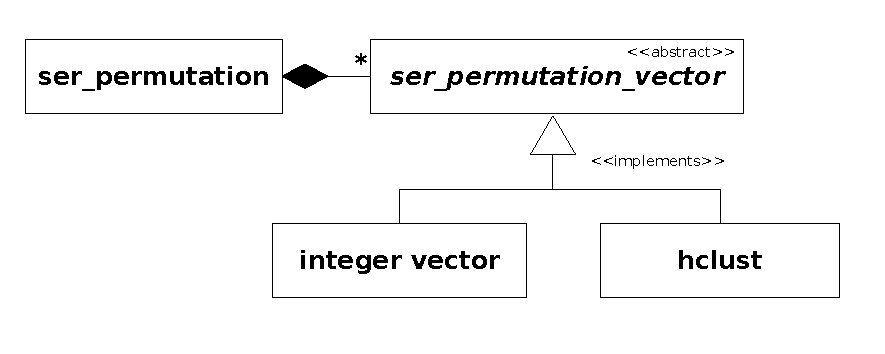
\includegraphics[width=10cm]{classes}}

    \caption{UML class diagram of the data structures for permutations provided by \pkg{seriation}}
    \label{fig:infrastructure}
\end{figure}

However, R provides no classes for representing permutation vectors.
\pkg{seriation} adds the necessary data structure (using the S3 class
system) as depicted in Figure~\ref{fig:infrastructure}. The class
\code{ser\_permutation} represents the permutation information for
$k$-mode data (including the cases of $k=1$ and $k=2$). It consists of
$k$ permutation vectors, where each permutation vector is represented by
an object of a concrete implementation of the abstract class
\code{ser\_permutation\_vector}.  This design is used to allow to use
arbitrary representations for the permutation vectors without removing
additional available information by just using an integer
vector. Currently, the permutation vector can be stored as a simple
integer vector or as an object of class \code{hclust} (defined in
package \pkg{stats}). \code{hclust} describes a hierarchical clustering
tree (dendrogram) including an ordering for the trees node leaves which
provides a permutation for all objects (see
Section~\ref{sec:hierarchical_clustering}).

Class \code{ser\_permutation\_vector} has a constructor
\func{ser\_permutation\_vector} which converts data into the correct concrete
subclass of \code{ser\_permutation\_vector} and checks if it contains a proper
permutation vector.  For \code{ser\_permutation\_vector} the methods
\func{print}, \func{length} for the length of the permutation vector,
\func{get\_method} to get the method used to generate the permutation, and
\func{get\_order} to access the raw (integer) permutation vector are available.
An accessor method \func{get\_order} is implemented for each concrete subclass
of \code{ser\_permutation\_vector}.  With this design, other classes
representing permutations can be easily incorporated by just adding an
appropriate \func{get\_order} methods for the new class.

For \code{ser\_permutation} a constructor is provided which can bind $k$
\code{ser\_permutation\_vector} objects together into an object for $k$-mode
data. \code{ser\_permutation} is implemented as a list of length~$k$ and each
element contains a \code{ser\_permutation\_vector} object.  Methods like
\func{length}, accessing elements with \code{[[}, \code{[[<-}, subsetting
with \code{[}, and combining  with \func{c} work as expected.  Also a
\func{print} method are provided. Finally, direct access to the raw permutation
vectors is available using \func{get\_order}.  Here the second argument (which
defaults to $1$) specifies the dimension (mode) for which the order vector is
requested.

All seriation algorithms are available via the function \func{seriate}
defined as:
\begin{quotation}
\code{seriate(x,  method = NULL, control = NULL, ...)}
\end{quotation}
where \code{x} is the input data, \code{method} is a string defining the
seriation method to be used and \code{control} can contain a list with
additional information for the algorithm.  \func{seriate} returns an object
of class \code{ser\_permutation} with a length conforming to the number of
dimensions of~\code{x}.  For \code{matrix} the additional argument
\code{margin} can be used if only column (\code{margin = 1}) or row seriation
(\code{margin = 2}) is needed.

%\begin{landscape}
\begin{table}[t]
\centering
    \begin{tabular}{lllc}
        \hline
Algorithm & \code{method} argument & Optimizes & Input data \\
        \hline
Simulated annealing & \code{"ARSA"} & Gradient measure &\code{dist} \\
Branch-and-bound & \code{"BBURCG"} & Gradient measure &\code{dist} \\
Branch-and-bound & \code{"BBWRCG"} & Gradient measure (weighted)& \code{dist} \\
TSP solver & \code{"TSP"} & Hamiltonian path length& \code{dist} \\
Rank-two ellipse seriation  & \code{"Chen"} & Other& \code{dist} \\
MDS -- first dimension & \code{"MDS"} & Other& \code{dist} \\
Hierarchical clustering & \code{"HC"} & Other& \code{dist} \\
Gruvaeus and Wainer & \code{"GW"} & Other& \code{dist} \\
Optimal leaf ordering  & \code{"OLO"} & 
    Hamiltonian path length (restricted)& \code{dist} \\
Bond Energy Algorithm & \code{"BEA"} &
    Measure of effectiveness & \code{matrix} \\
TSP to optimize ME & \code{"BEA\_TSP"} &
    Measure of effectiveness& \code{matrix} \\
First principal component & \code{"PCA"} & 
    Other& \code{matrix} \\
        \hline
    \end{tabular}
    \caption{Currently implemented methods for \func{seriation}.}
\label{tab:methods}
\end{table}
%\end{landscape}

Various seriation methods were already introduced in this paper in
Section~\ref{sec:methods}. In Table~\ref{tab:methods} we summarize the methods
currently available in the package for seriation.  The code for the simulated
annealing heuristic~\citep{seriation:Brusco:2007} and the two
branch-and-bound~\citep{seriation:Brusco:2005} was obtained from the authors.
The TSP solvers (exact solvers and a variety of heuristics) is provided by
package \pkg{TSP}~\citep{seriation:Hahsler:2007}.  For the rank-two ellipse
seriation we implemented the algorithm by~\cite{seriation:Chen:2002}.  For the
Gruvaeus and Wainer algorithm, the implementation in package
\pkg{gclus}~\citep{seriation:Hurley:2007} is used.  For optimal leaf ordering we
implemented the algorithm by~\cite{seriation:Bar-Joseph:2001}.  The BEA code
was kindly provided by Fionn Murtagh.  Over time more methods will be added to
the package.

To calculate the value of a loss/merit function for data and 
a certain permutation, the function
\begin{quotation}
\code{criterion(x, order = NULL, method = "all", ...)} 
\end{quotation}
is provided. \code{x} is the data object, \code{order} contains a suitable
object of class \code{ser\_permutation} (if omitted no permutation is
performed) and \code{method} specifies the type of loss/merit function. A
vector of several methods can be used resulting in a named vector
with the values of the requested functions.  We already
defined different loss/merit functions for seriation in
Section~\ref{sec:seriation}.  In Table~\ref{tab:criteria} we indicate the
loss/merit functions currently available in the package.  Additionally, the
pseudo method \code{"all"} (which is the default) can be used to calculate
the values for all applicable loss/merit functions.

\begin{table}[t]
\centering
\begin{tabular}{llcc}
        \hline
        Name & \code{method} argument & merit/loss & Input data \\
        \hline
        Anti-Robinson events& \code{"AR\_events"} & 
loss & \code{dist} \\
        Anti-Robinson deviations& \code{"AR\_deviations"} & 
loss & \code{dist} \\
        Gradient measure& \code{"Gradient\_raw"} & 
merit & \code{dist} \\
        Gradient measure (weighted)& \code{"Gradient\_weighted"} & 
merit & \code{dist} \\
        Hamiltonian path length & \code{"Path\_length"} & loss & \code{dist} \\
        Inertia criterion& \code{"Inertia"} & merit & \code{dist} \\
        Least squares criterion& \code{"Least\_squares"} & loss & \code{dist} \\
        Measure of effectiveness& \code{"ME"} & 
merit & \code{matrix} \\
        Stress (Moore neighborhood)& \code{"Moore\_stress"} & 
loss & \code{matrix} \\
        Stress (Neumann neighborhood)& \code{"Neumann\_stress"} & 
loss & \code{matrix} \\
        \hline
    \end{tabular}
    \caption{Implemented loss/merit functions in function \func{criterion}.}
\label{tab:criteria}
\end{table}

In addition the package offers the (generic) function
\begin{quotation}
\code{permute(x, order)} 
\end{quotation}
where \code{x} is the data (a \code{dist} object, a matrix, an
array, a list or a numeric vector) to be reordered and \code{order} is a
\code{ser\_permutation} object of suitable length. 
%The permutation for
%\code{dist} objects uses package \pkg{proxy}~\citep{seriation:Meyer:2007}.

For visualization, the package offers several options:
\begin{itemize}
\item Matrix shading with \func{pimage}. In contrast to the 
        standard \func{image} in package~\pkg{graphics}, \func{pimage}
        displays the matrix as is with the first element in the top
        left-hand corner and using a gamma-corrected gray scale.

\item Different heat maps (e.g., with optimally reordered
    dendrograms) with \func{hmap}.

\item Visualization of data matrices in the spirit 
of~\cite{seriation:Bertin:1981} with \func{bertinplot}.

\item \emph{Dissimilarity plot}, a new visualization to judge the
    quality of a clustering using matrix shading 
    and seriation with \func{dissplot}.
\end{itemize}

We will introduce the package usage and the visualization options
in the examples in the next section.

\section{Examples and applications}
\label{sec:example}


We start this section with a simple first session to demonstrate the basic
usage of the package. Then we present and discuss several seriation 
applications.

\subsection{A first session using \pkg{seriation}}
In the following example, we use the well known iris data set
(from R's \pkg{datasets} package) which gives the
measurements in centimeters of the variables sepal length and width and petal
length and width, respectively, for 50 flowers from each of 3 species of the
iris family (Iris setosa, versicolor and virginica). 

First, we load the package \pkg{seriation} and the iris data set.  We
remove the species classification and reorder the objects randomly since
they are already sorted by species in the data set. Then we calculate
the Euclidean distances between objects.

\begin{Schunk}
\begin{Sinput}
> library("seriation")
> data("iris")
> x <- as.matrix(iris[-5])
> x <- x[sample(seq_len(nrow(x))), ]
> d <- dist(x)
\end{Sinput}
\end{Schunk}

To seriate the objects given the dissimilarities, we just call
\func{seriate} with the default settings.

\begin{Schunk}
\begin{Sinput}
> order <- seriate(d)
> order
\end{Sinput}
\begin{Soutput}
object of class ‘ser_permutation’, ‘list’
contains permutation vectors for 1-mode data

  vector length seriation method
1           150             ARSA
\end{Soutput}
\end{Schunk}

The result is an object of class \code{ser\_permutation} for 
one-mode data. The permutation vector length is $150$ for the
$150$ objects in the iris data set and the used seriation method is
\code{"ARSA"}, a simulated annealing heuristic
(see~Table~\ref{tab:methods}).

To visually inspect the effect of seriation on the distance matrix, we use
matrix shading with \func{pimage} (the result is shown in 
Figure~\ref{fig:pimage1}).

\begin{Schunk}
\begin{Sinput}
> pimage(d, main = "Random")
> pimage(d, order, main = "Reordered")
\end{Sinput}
\end{Schunk}
\begin{figure}
    \centering
    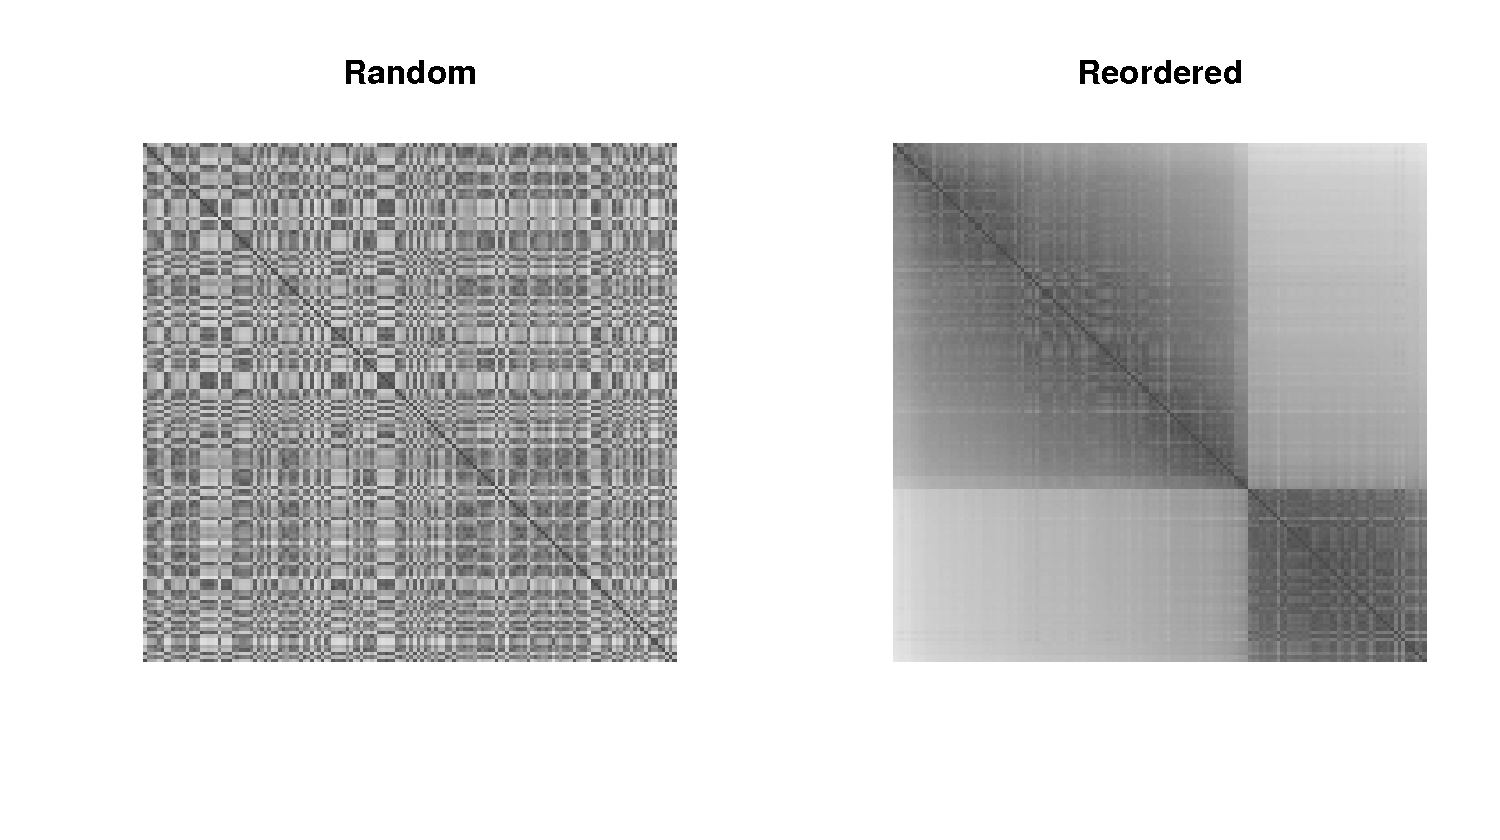
\includegraphics[width=12cm]{seriation-pimage1}
    \caption{Matrix shading of the  distance matrix for the iris data.}
    \label{fig:pimage1}
\end{figure}

Finally, we can also compare the improvement for different loss functions
using \func{criterion}.

\begin{Schunk}
\begin{Sinput}
> cbind(random = criterion(d), reordered = criterion(d, order))
\end{Sinput}
\begin{Soutput}
                       random    reordered
AR_events            551693.0     54915.00
AR_deviations        943320.0      9442.40
Gradient_raw          -1392.0    992073.00
Gradient_weighted      9153.5   1772117.91
Path_length             359.5        86.44
Inertia           215367939.3 356947608.76
Least_squares      78838267.7  76487648.47
ME                   301406.5    402260.78
Moore_stress         885654.0     14060.78
Neumann_stress       415557.8      5556.31
\end{Soutput}
\end{Schunk}

Naturally, the reordered dissimilarity matrix achieves better values for all
criteria (note that the measure of effectiveness and inertia 
are merit functions and larger values are better).

Also the original data matrix can be easily inspected using \func{pimage}.
To use the result of the seriation for the original two-mode data,
we have to add a permutation vector to the \code{ser\_permutation}
object. To leave the columns in the original order, we add an 
identity permutation vector to the permutations object using the combine 
function \func{c}. 

\begin{Schunk}
\begin{Sinput}
> pimage(x, main = "Random")
> order_2mode <- c(order, ser_permutation(seq_len(ncol(x))))
> order_2mode
> pimage(x, order_2mode, main = "Reordered")
\end{Sinput}
\end{Schunk}
\begin{Schunk}
\begin{Soutput}
object of class ‘ser_permutation’, ‘list’
contains permutation vectors for 2-mode data

  vector length seriation method
1           150             ARSA
2             4          unknown
\end{Soutput}
\end{Schunk}
\begin{figure}
    \centering
    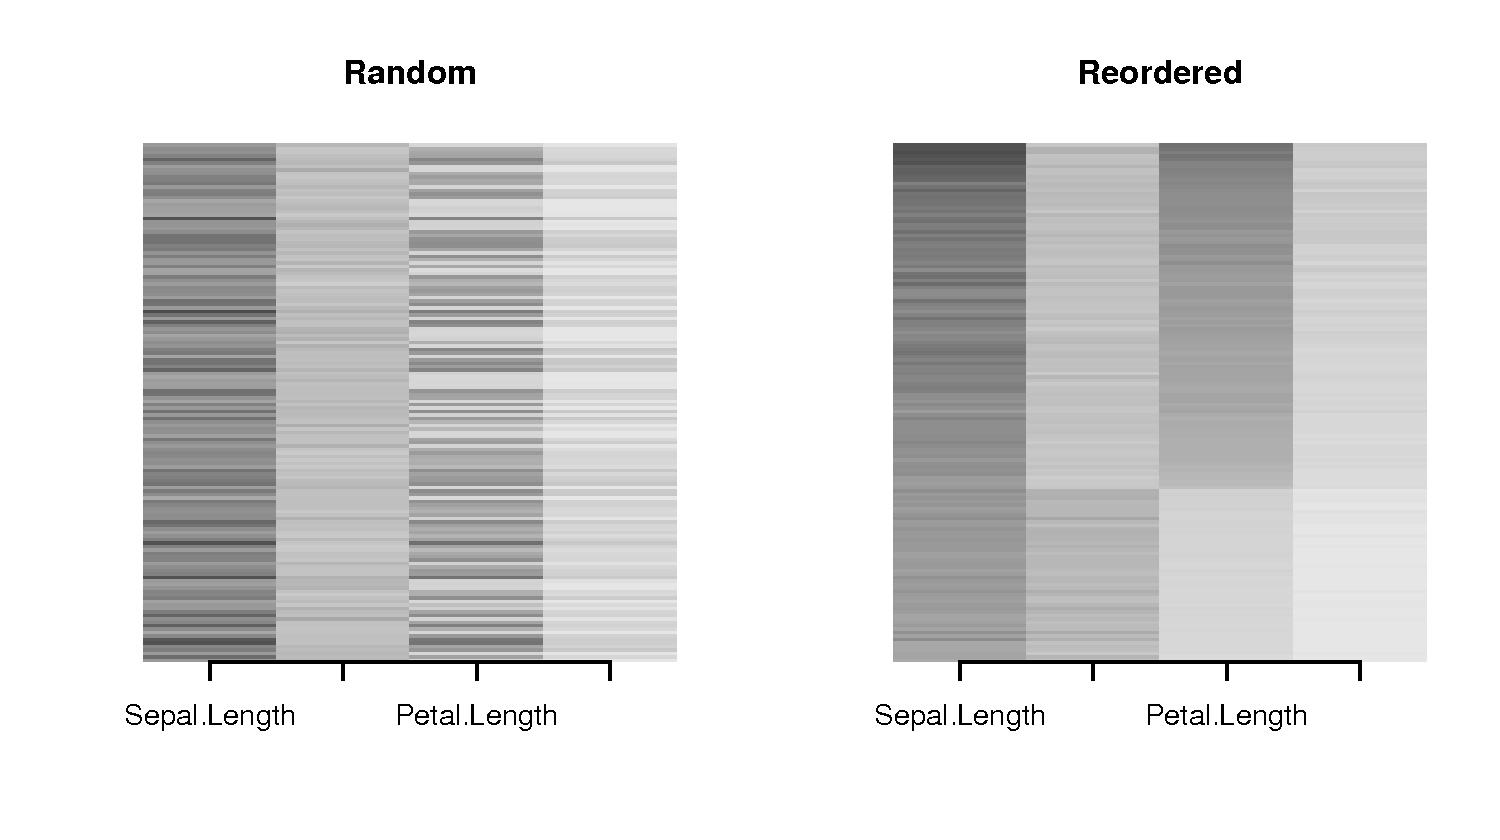
\includegraphics[width=12cm]{seriation-pimage2}
    \caption{Matrix shading of the iris data matrix.}
    \label{fig:pimage2}
\end{figure}

\subsection{Comparing different seriation methods}

To compare different seriation methods we use again the randomized iris data
set and the distance matrix \code{d} from the previous example.  We include in
the comparison several seriation methods for dissimilarity matrices described
in Section~\ref{sec:methods}. 

\begin{Schunk}
\begin{Sinput}
> methods <- c("TSP", "Chen", "ARSA", "HC", "GW", "OLO")
> order <- sapply(methods, FUN = function(m) seriate(d, m), 
+     simplify = FALSE)
\end{Sinput}
\end{Schunk}

The resulting orderings are displayed using matrix shading
(see Figure~\ref{fig:pimage3}).
\begin{Schunk}
\begin{Sinput}
> tmp <- lapply(order, FUN = function(o) pimage(d, o, main = get_method(o[[1]])))
\end{Sinput}
\end{Schunk}

\begin{figure}
    \centering
    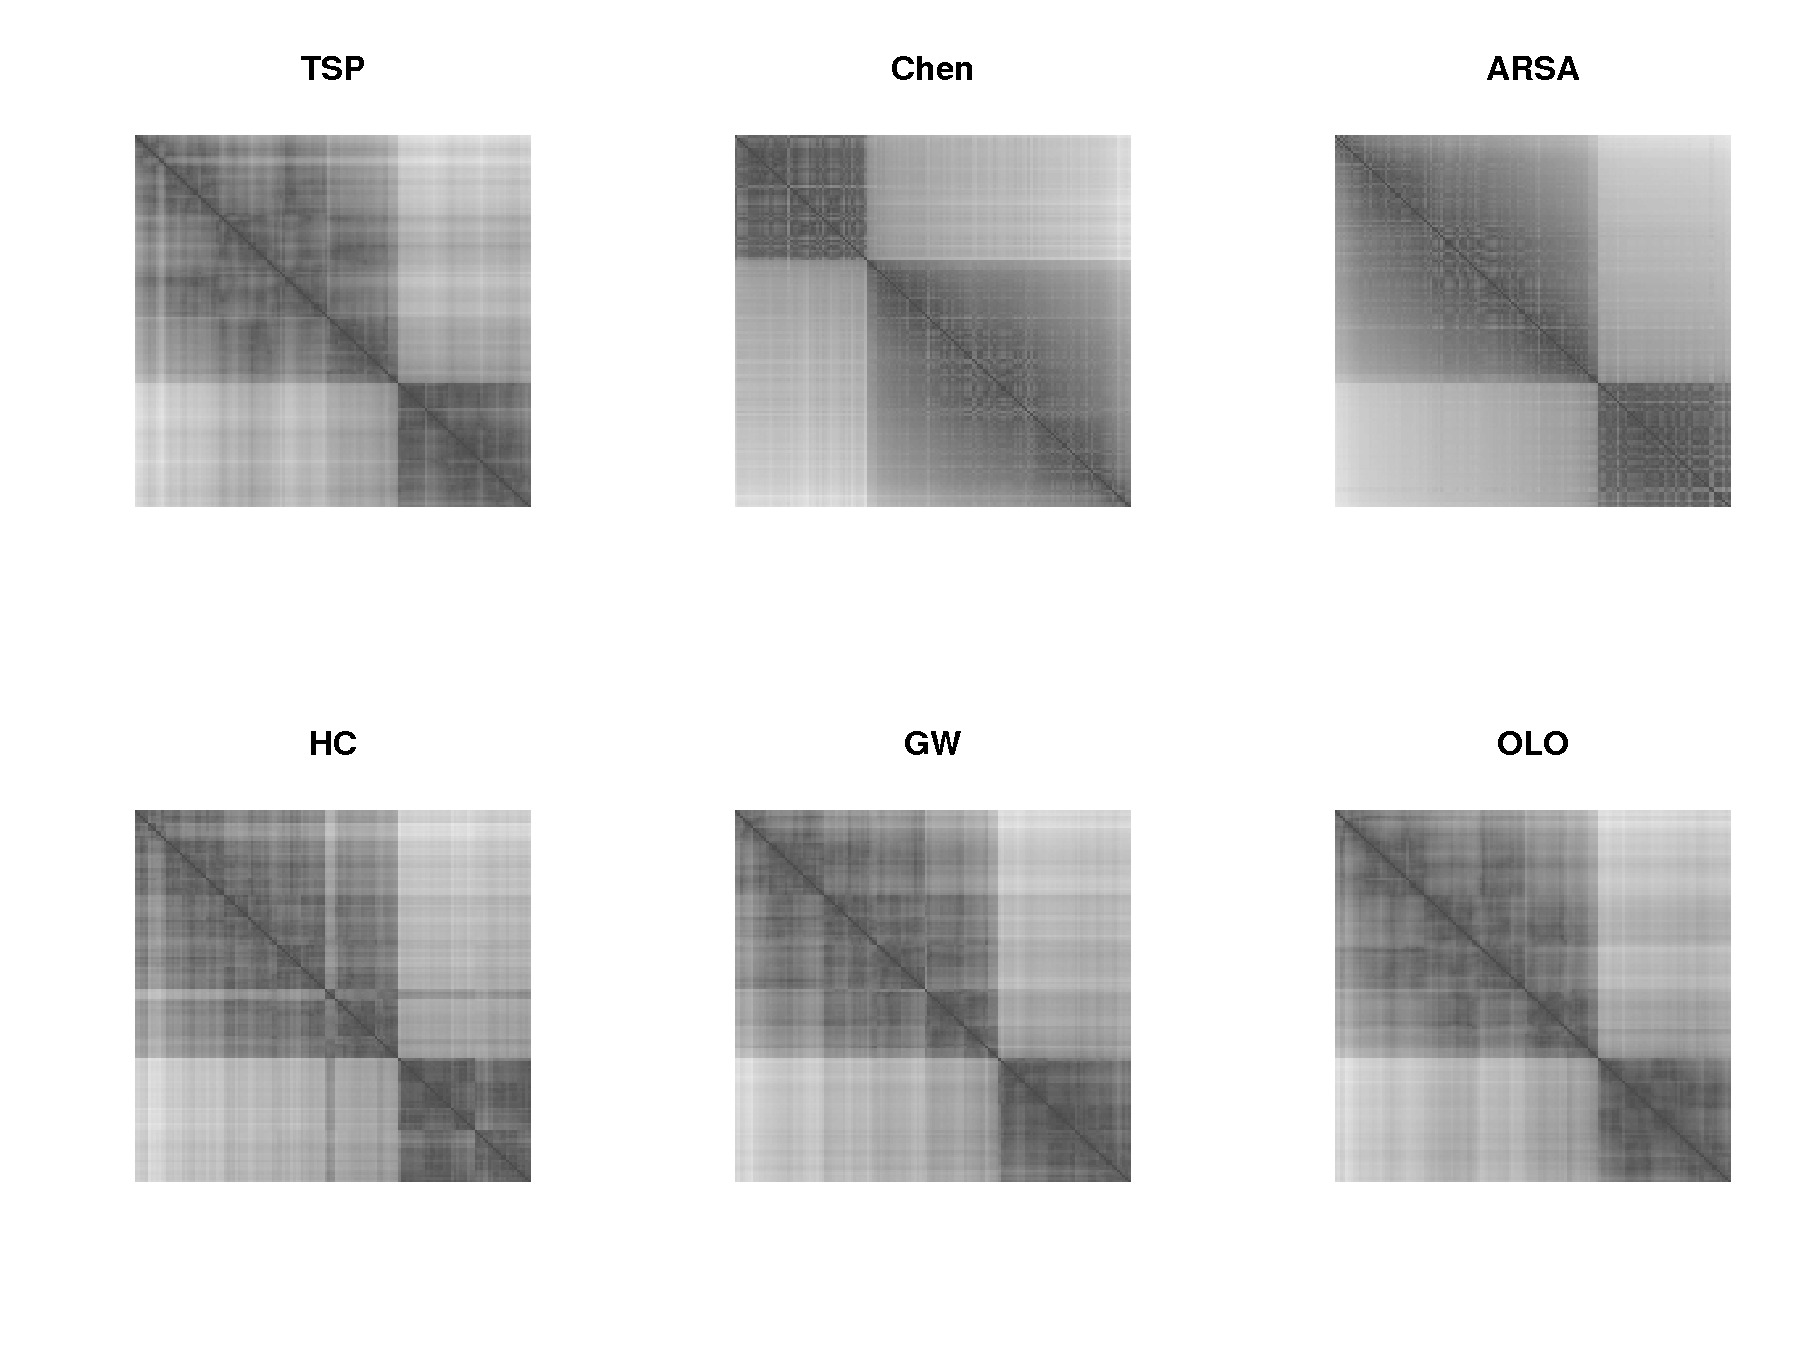
\includegraphics[width=\linewidth]{seriation-pimage3}
    \caption{Image plot of the distance matrix for the iris data
    using rearrangement by different seriation methods.}
    \label{fig:pimage3}
\end{figure}

Finally, we compare the values of the loss/merit functions 
for the different seriation methods. 
\begin{Schunk}
\begin{Sinput}
> crit <- sapply(order, FUN = function(o) criterion(d, o))
> t(crit)
\end{Sinput}
\begin{Soutput}
     AR_events AR_deviations Gradient_raw Gradient_weighted Path_length
TSP     165453         51174       770981           1651215       52.41
Chen     90015         18184       921885           1746766       85.43
ARSA     55010          9424       991884           1772114       85.44
HC      173729         53167       754425           1644981       64.15
GW      171903         44776       758071           1664667       57.24
OLO     174625         46900       752619           1660309       51.11
       Inertia Least_squares     ME Moore_stress Neumann_stress
TSP  345485410      76648852 402674        15294           5238
Chen 354057418      76521451 402018        19358           7305
ARSA 356944288      76487654 402346        13333           5217
HC   345722302      76657164 402560        30347          10401
GW   346564518      76630917 402822        18636           6426
OLO  346172124      76636726 403053        14979           5126
\end{Soutput}
\end{Schunk}


\begin{figure}
    \centering
    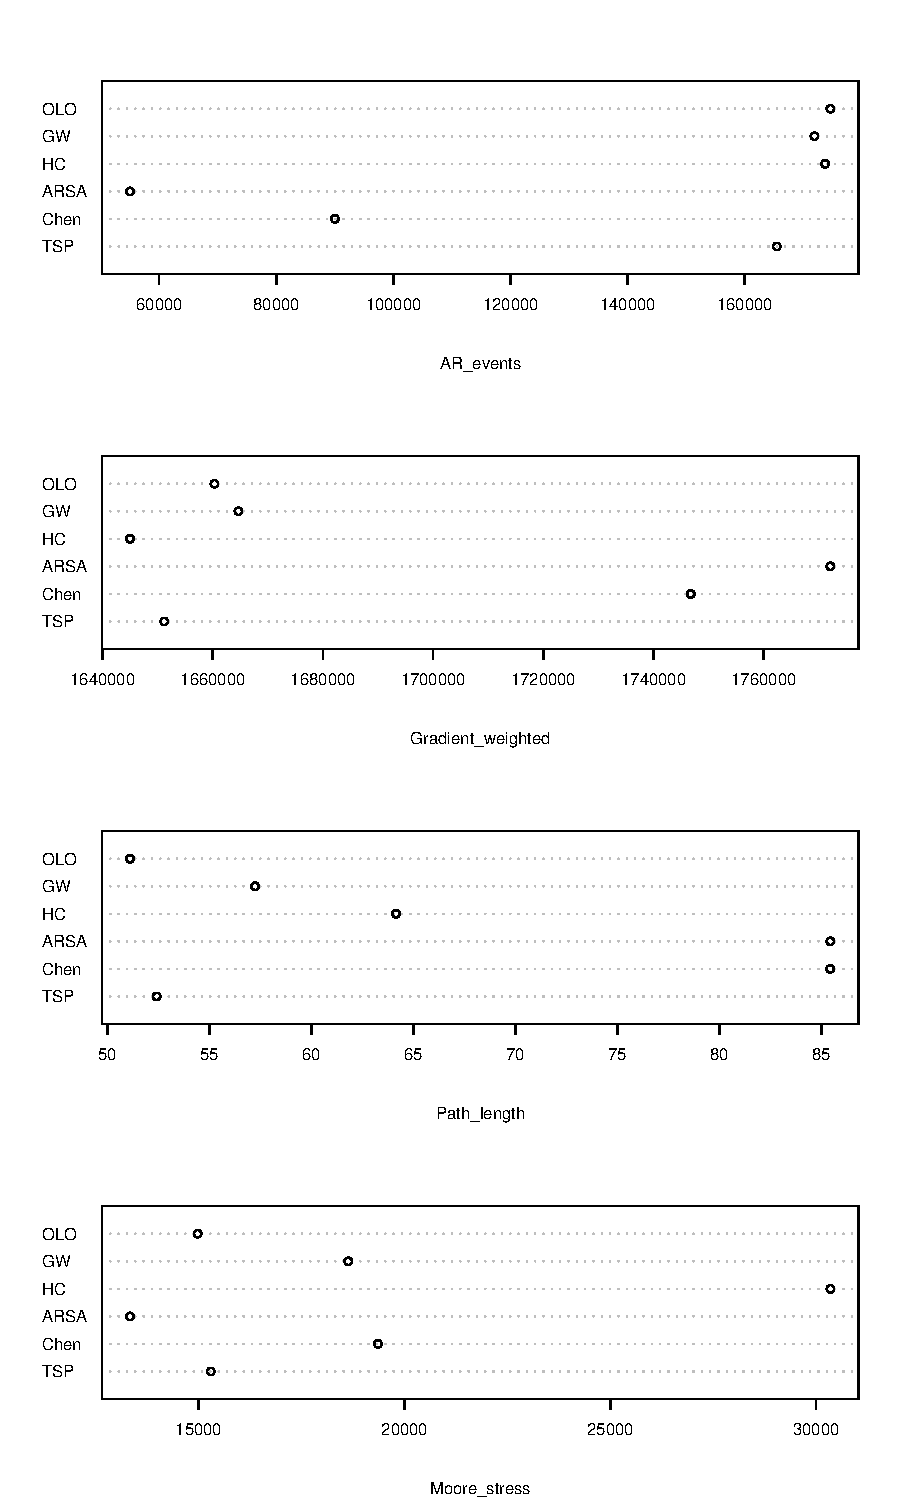
\includegraphics{seriation-crit1}
    \caption{Comparison of different methods and seriation criteria}
    \label{fig:crit1}
\end{figure}

For easier comparison, Figure~\ref{fig:crit1} contains a plot of the criteria
Hamiltonian path length, anti-Robinson events (\code{AR\_events}) and stress
using the Moore neighborhood. Clearly, the methods which directly try to
minimize the Hamiltonian path length (hierarchical clustering with optimal leaf
ordering (\code{OLO}) and the TSP heuristic) provide the best results
concerning the path length. For the number of anti-Robinson events, using the
simulated annealing heuristic (\code{ARSA}) provides the best result since it
directly aims at minimizing this loss function.  Regarding stress, the
simulated annealing heuristic also provides the best result although, it does
not directly minimize this loss function.


\subsection{Heat maps}

A heat map is a shaded/color coded data matrix with a dendrogram added to one
side and to the top to indicate the order of rows and columns. Typically,
reordering is done according to row or column means within the restrictions
imposed by the dendrogram. Heat maps recently became popular for visualizing
large scale genome expression data obtained via DNA microarray technology
\citep[see, e.g.,][]{seriation:Eisen:1998}. 

From Section~\ref{sec:hierarchical_clustering} we know that it is possible to
find the optimal ordering of the leaf nodes of a dendrogram which minimizes
the distances between adjacent objects in reasonable time.  Such an order might
provide an improvement over using simple reordering such as the row or column
means with respect to presentation. In \pkg{seriation} we provide
the function \func{hmap} which uses optimal ordering and can also use 
seriation directly on distance matrices without using hierarchical
clustering to produce dendrograms first.

For the following example, we use again the randomly reordered iris data set
\code{x} from the examples above. To make the variables (columns) comparable,
we use standard scaling.

\begin{Schunk}
\begin{Sinput}
> x <- scale(x, center = FALSE)
\end{Sinput}
\end{Schunk}

To produce a heat map with optimally reordered dendrograms, the function
\func{hmap} can be used with its default settings. With these settings, the
Euclidean distances between rows and between columns are calculated (with
\func{dist}), hierarchical clustering (\func{hclust}) is performed, the
resulting dendrograms are optimally reordered, and \func{heatmap} in package
\pkg{stats} is used for plotting. 
\begin{Schunk}
\begin{Sinput}
> hmap(x)
> hmap(x, hclustfun = NULL)
\end{Sinput}
\end{Schunk}
(see Figure~\ref{fig:heatmap}).

If \code{hclustfun = NULL} is used, instead of hierarchical clustering,
seriation on the dissimilarity matrices for rows and columns is
performed (using a TSP heuristic by default) and the reordered matrix
with the reordered dissimilarity matrices to the left and on top is
displayed.  A \code{method} argument can be used to choose different
seriation methods.


\begin{figure}
    \begin{minipage}[b]{.48\linewidth}
        \centering
        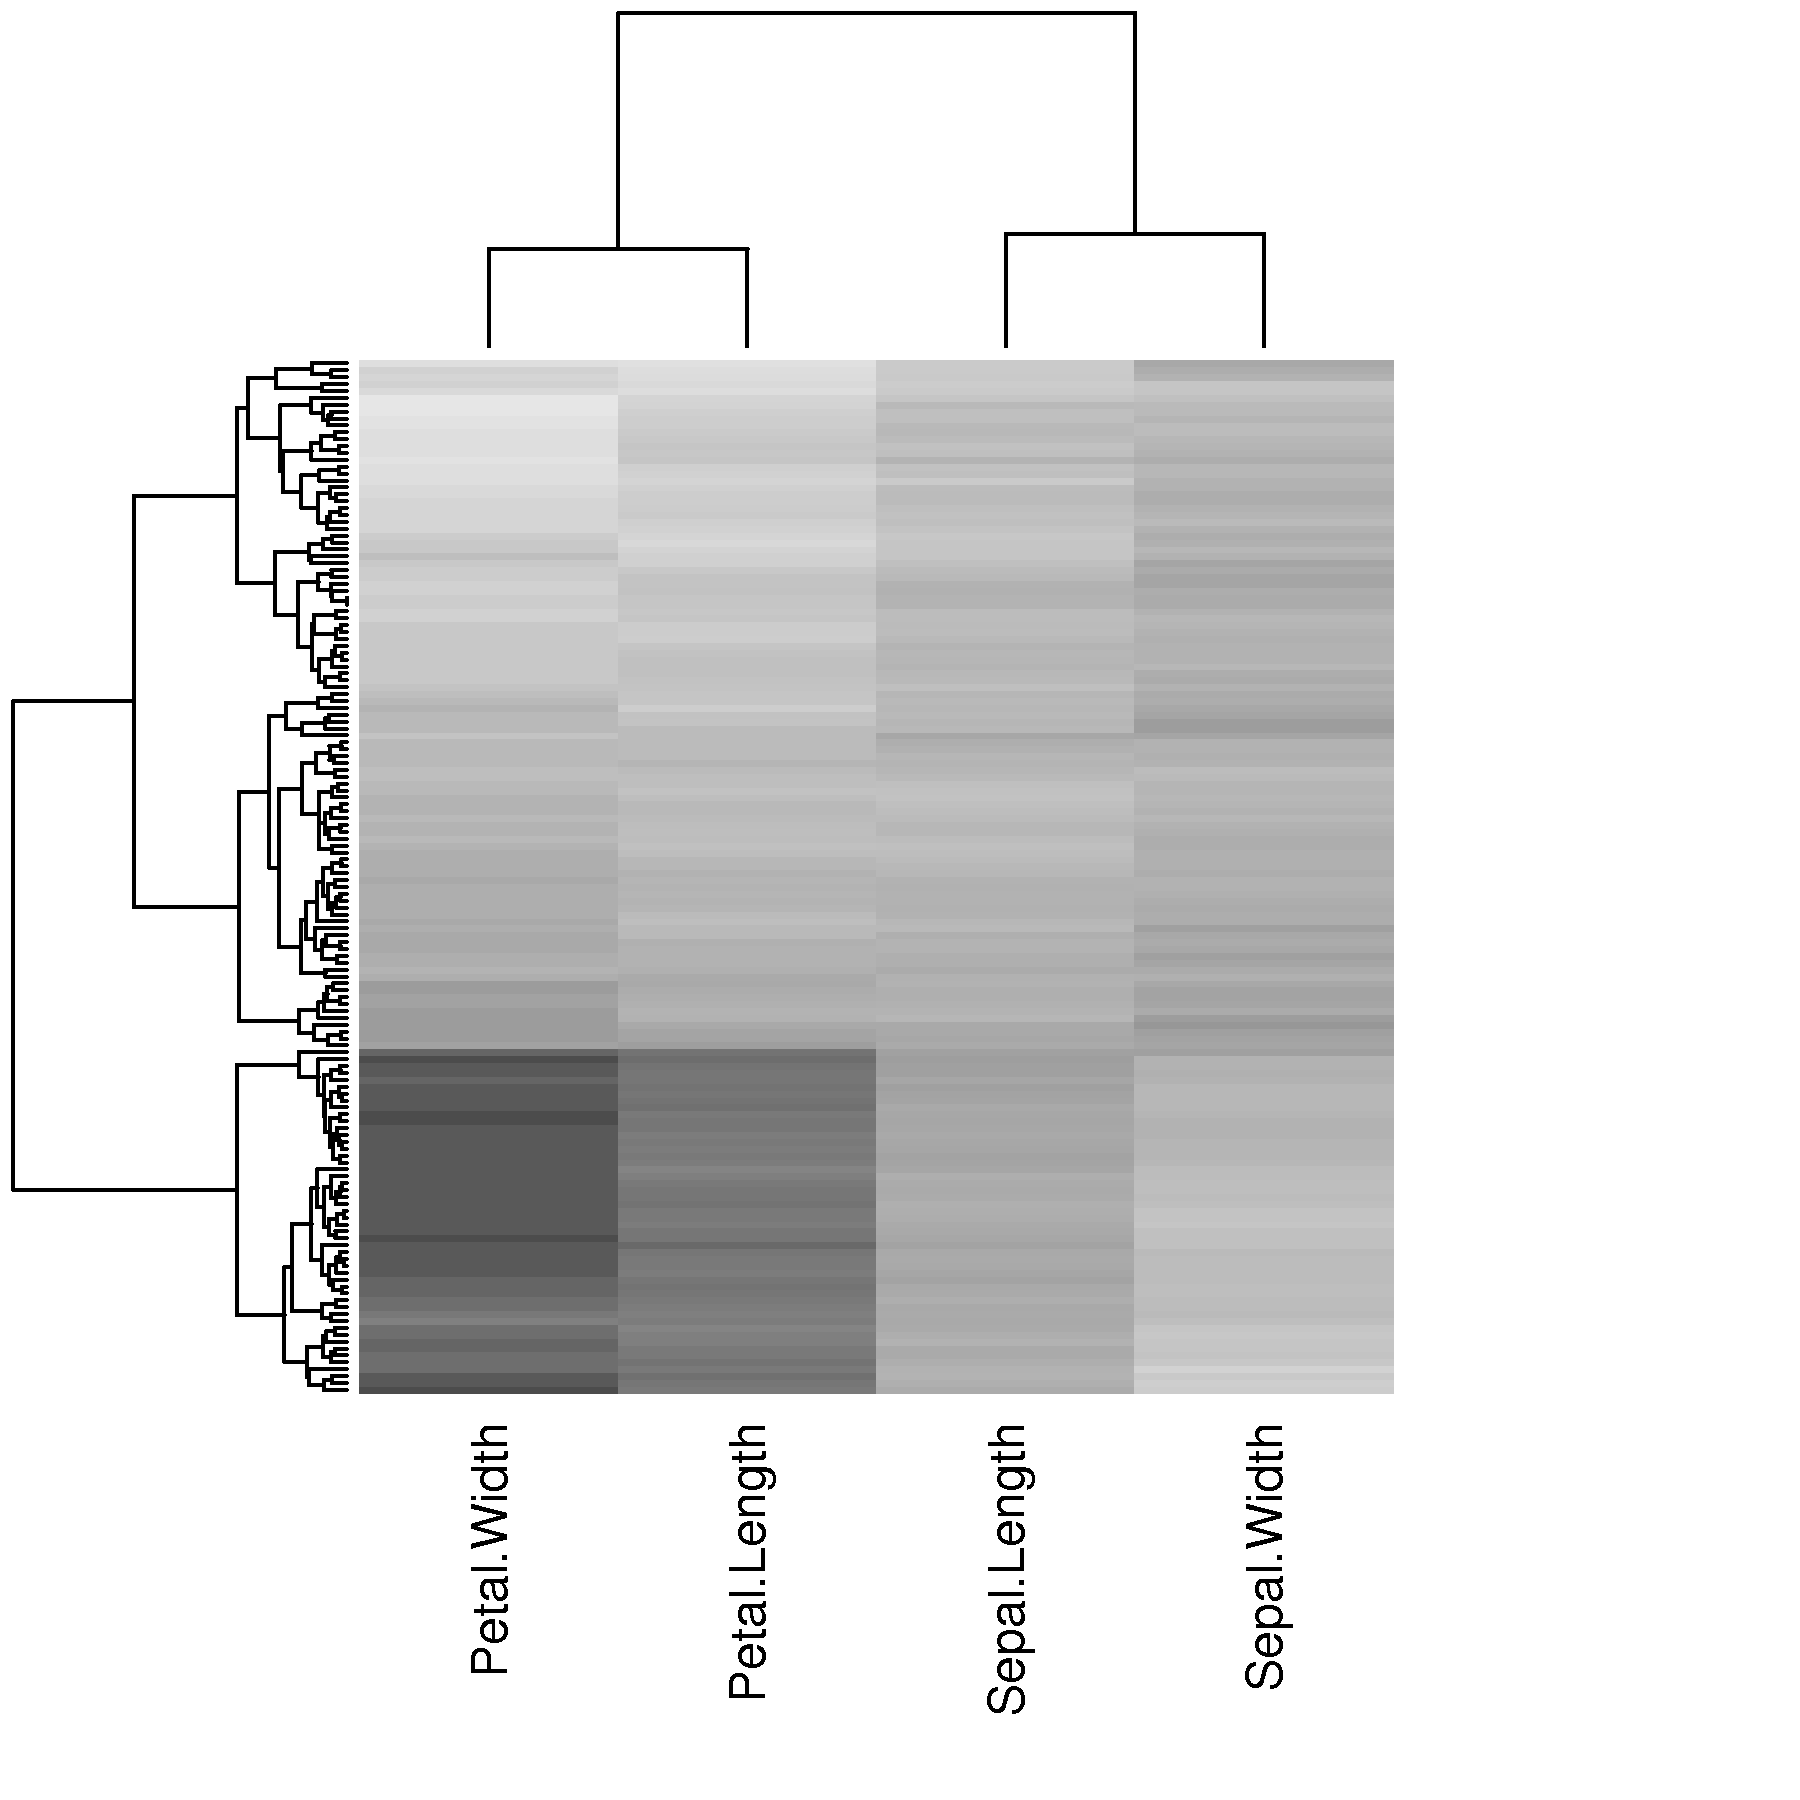
\includegraphics[width=\linewidth]{seriation-heatmap1} \\
            (a)
    \end{minipage}
    \begin{minipage}[b]{.48\linewidth}
        \centering
        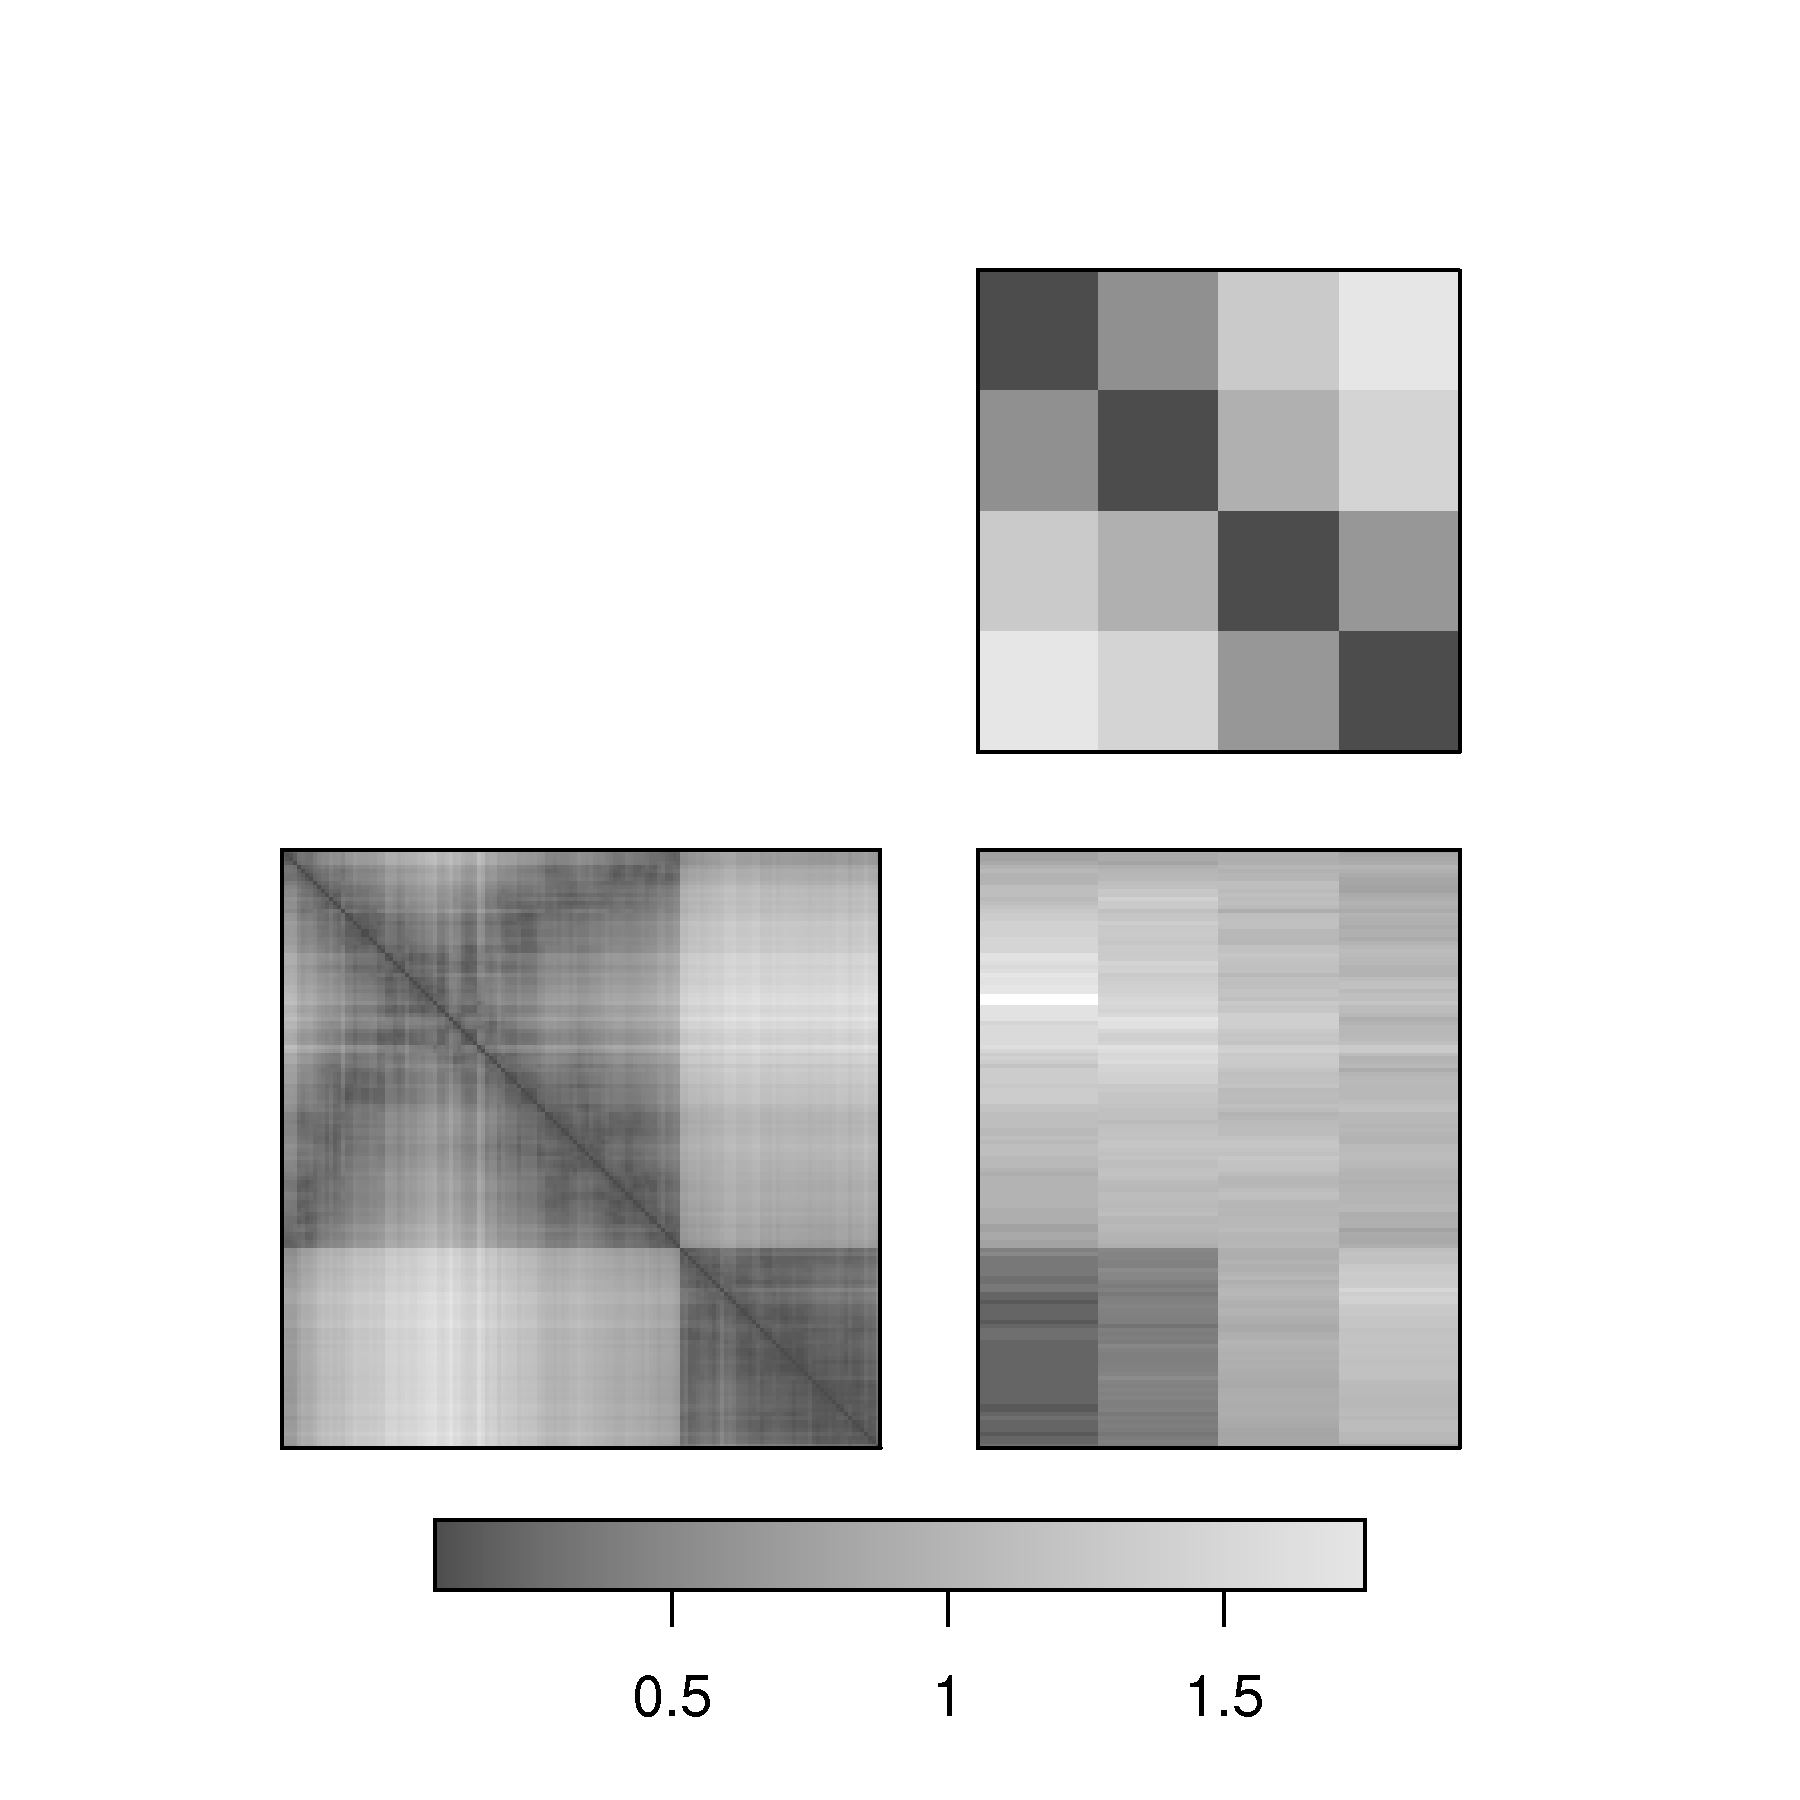
\includegraphics[width=\linewidth]{seriation-heatmap2} \\
            (b)
    \end{minipage}
    \caption{Two presentations of the rearranged iris data matrix. (a) as an
optimally reordered heat map and (b) as a seriated data matrix with reordered
dissimilarity matrices to the left and on top.}
    \label{fig:heatmap}
\end{figure}


\subsection{Bertin's permutation matrix}

\cite{seriation:Bertin:1981,seriation:Bertin:1999} 
introduced permutation matrices to analyze
multivariate data with medium to low sample size.  The idea is to reveal a more
homogeneous structure in a data matrix $\mathbf{X}$ by simultaneously
rearranging rows and columns. The rearranged matrix is displayed and cases and
variables can be grouped manually to gain a better understanding of the data.

To quantify homogeneity, a purity function
\begin{displaymath}
  \phi = \Phi(\mathbf{X})  
\end{displaymath}
is defined. Let $\Pi$ be the set of all permutation functions
$\pi$ for matrix $\mathbf{X}$.
Note that function $\pi$ performs row and column permutations on a matrix.
The optimal permutation with respect to
purity
\begin{displaymath}
  \pi^* = \argmax\nolimits_{\pi \in \Pi} \Phi(\pi(\mathbf{X}))  
\end{displaymath}
is found and the rearranged matrix $\pi(\mathbf{X})$ is
displayed. Since, depending on the purity function, finding the optimal
solution can be hard, often a near optimal solution is also acceptable.

A possible purity function $\Phi$ is:
Given distances between rows and columns of the data matrix, define purity as
the sum of distances of adjacent rows/columns.  Using this purity function,
finding the optimal permutation $\pi^*$ means solving two (independent) TSPs,
one for the columns and one for the rows.

As an example, we use the results of $8$ constitutional referenda for $41$
Irish communities~\citep{seriation:Falguerolles:1997}\footnote{The Irish data
set is included in this package. The original data and the text of the
referenda can be obtained from~\url{http://www.electionsireland.org/}}.  To
make values comparable across columns (variables), the ranks of the values for
each variable are used instead of the original values.  

\begin{Schunk}
\begin{Sinput}
> data("Irish")
> orig_matrix <- apply(Irish[, -6], 2, rank)
\end{Sinput}
\end{Schunk}

For seriation, we calculate distances between rows and between columns using
the sum of absolute rank differences (this is equal to the Minkowski distance
with power $1$). Then we apply seriation (using a TSP heuristic) to both
distance matrices and combine the two resulting \code{ser\_permutation} objects
into one object for two-mode data. The original and the reordered matrix are
plotted using \func{bertinplot}. 

\begin{Schunk}
\begin{Sinput}
> order <- c(seriate(dist(orig_matrix, "minkowski", p = 1), 
+     method = "TSP"), seriate(dist(t(orig_matrix), "minkowski", 
+     p = 1), method = "TSP"))
> order
\end{Sinput}
\begin{Soutput}
object of class ‘ser_permutation’, ‘list’
contains permutation vectors for 2-mode data

  vector length seriation method
1            41              TSP
2             8              TSP
\end{Soutput}
\end{Schunk}



\begin{Schunk}
\begin{Sinput}
> bertinplot(orig_matrix)
> bertinplot(orig_matrix, order)
\end{Sinput}
\end{Schunk}
\begin{figure}
    \centering
    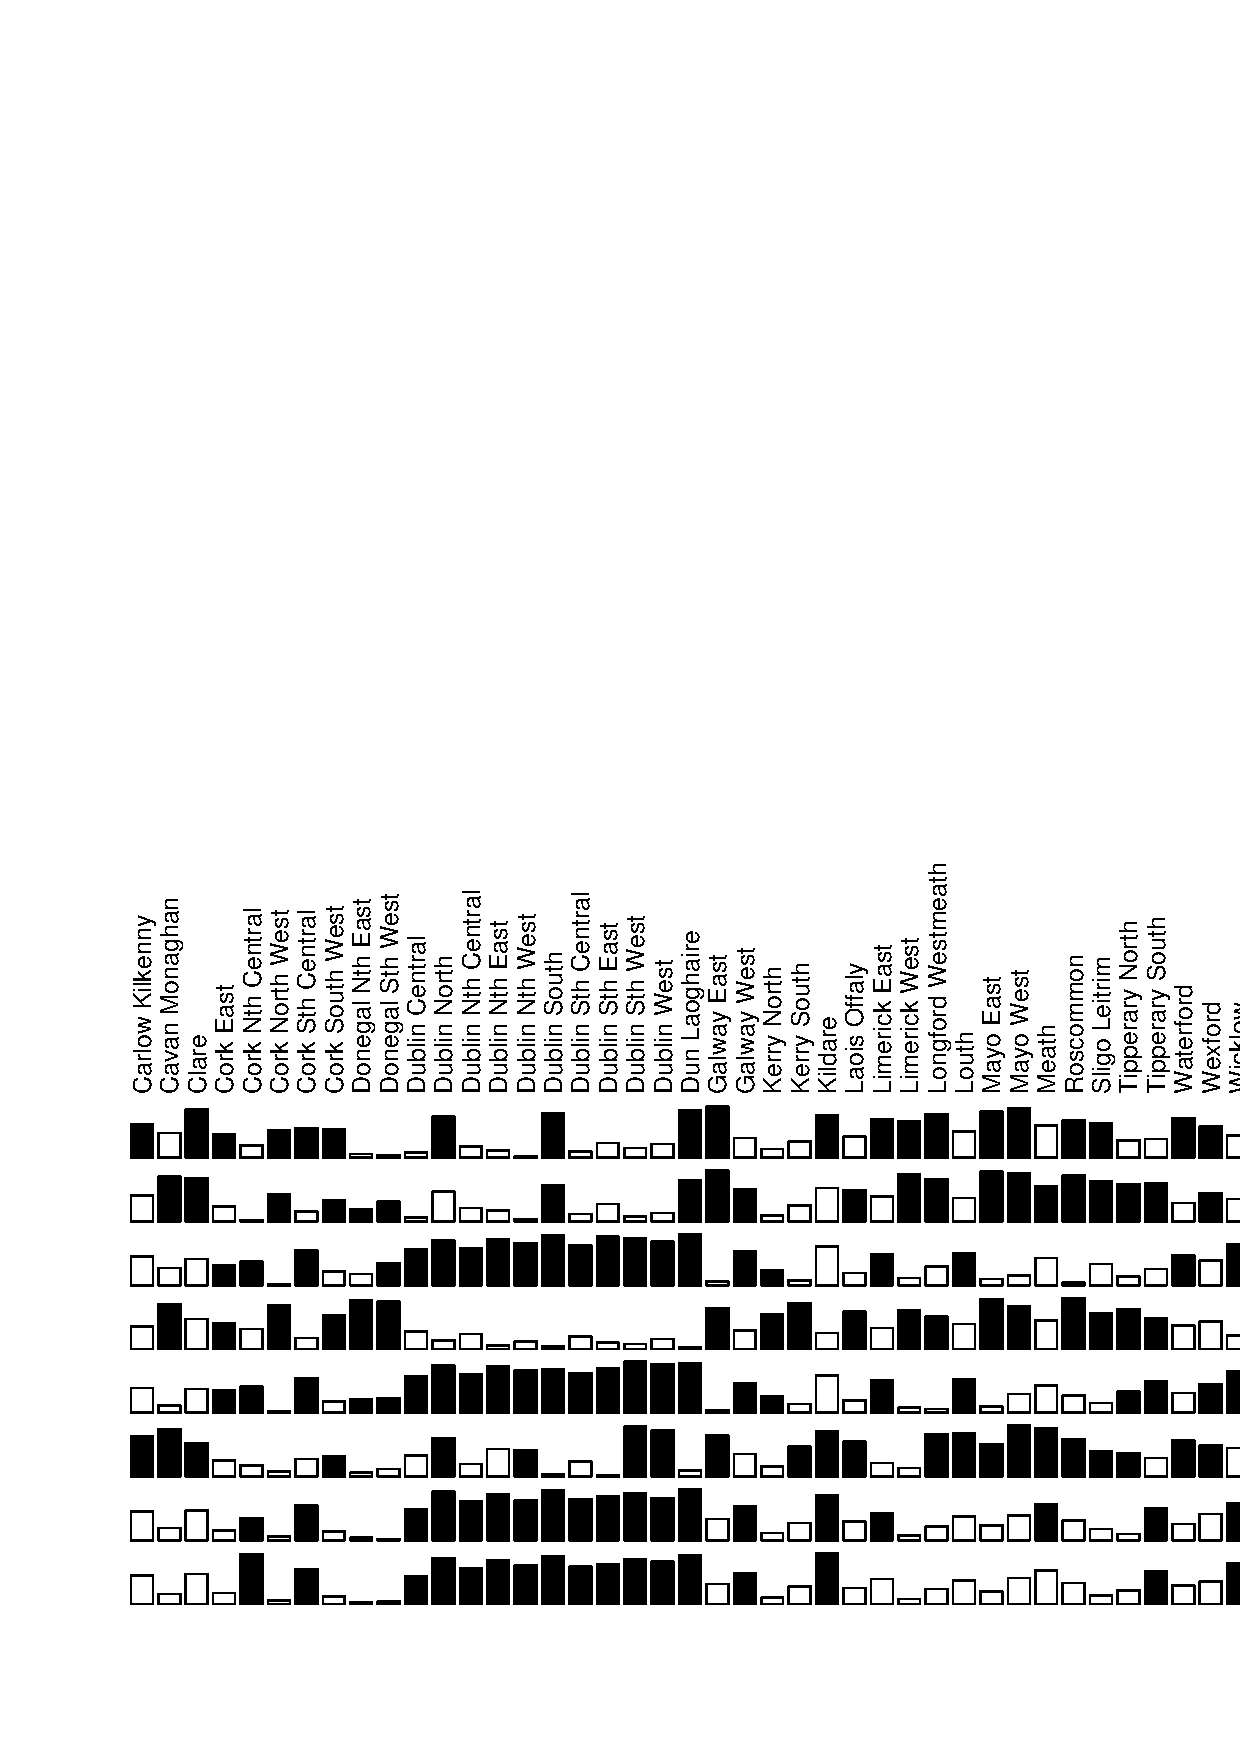
\includegraphics[width=15cm, trim=60 60 0 0]{seriation-bertin1} \\
    (a)
    
    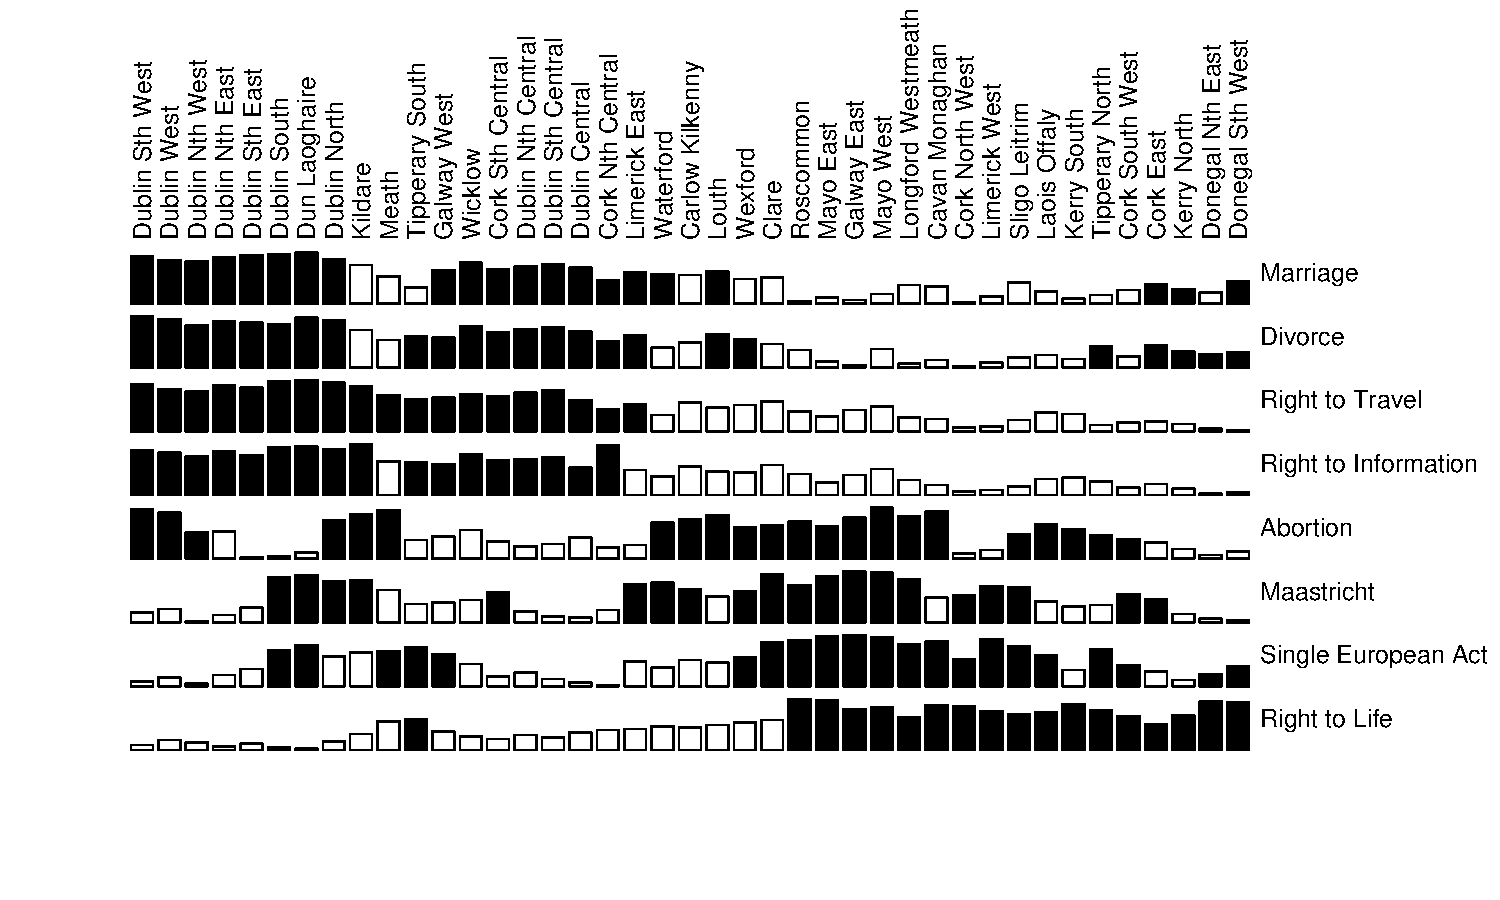
\includegraphics[width=15cm, trim=60 60 0 0]{seriation-bertin2} \\
    (b)    
    \caption{Bertin plot for the (a) original arrangement and the (b) 
    reordered Irish data set.}
    \label{fig:bertin}
\end{figure}



The original matrix and the rearranged matrix are shown in
Figure~\ref{fig:bertin} as a matrix of bars where high values are highlighted
(filled blocks).  Note that following Bertin, the cases (communities) are
displayed as the columns and the variables (referenda) as rows.  Depending on
the number of cases and variables, columns and rows can be exchanged to obtain
a better visualization.

Although the columns are already ordered (communities in the same city appear
consecutively) in the original data matrix in Figure~\ref{fig:bertin}(a), it
takes some effort to find structure in the data.  For example, it seems that
the variables `Marriage', `Divorce', `Right to Travel' and `Right to
Information' are correlated since the values are all high in the block made up
by the columns of the communities in Dublin.  The reordered matrix affirms this
but makes the structure much more apparent. Especially the contribution of low
values (which are not highlighted) to the overall structure becomes only
visible after rearrangement.

\subsection{Binary data matrices}

Binary or $0$-$1$ data matrices are quite common.  Often such matrices are
called \emph{incidence matrices} since a $1$ in a cell indicates the incidence
of an event. In archeology such an event could be that a special type of
artifact was found at a certain archaeological site.
This can be seen as a simplification of a so called \emph{abundance matrix}
which codes in each cell the (relative) frequency or quantity of an artifact
type at a site. For a comparison of incidence and abundance matrices
in archeology we refer the reader to~\cite{seriation:Ihm:2005}. 

Here we are interested in binary data.
For the example we use an artificial data set from~\cite{seriation:Bertin:1981}
called \emph{Townships}.  The data set contains $9$ binary characteristics
(e.g., has a veterinary or has a high school) for $16$ townships. The idea of
the data set is that townships evolve from a rural to an urban environment over
time.

After loading the data set (which comes with the package), we use
\func{bertinplot} to visualize the data (\func{pimage} could also be used
but \func{bertinplot} allows for a nicer visualization).
Bars, the standard visualization of \func{bertinplot}, do not
make much sense for binary data. We therefore use the 
panel function \func{panel.squares} without spacing 
to plot black squares.

\begin{Schunk}
\begin{Sinput}
> data("Townships")
> bertinplot(Townships, options = list(panel = panel.squares, 
+     spacing = 0, frame = TRUE))
\end{Sinput}
\end{Schunk}

The original data in Figure~\ref{fig:binary}(a) does not reveal structure in
the data. To improve the display, we run the  bond energy algorithm (BEA) for
columns and rows $10$ times with random starting points and report the best
solution. 


\begin{Schunk}
\begin{Sinput}
> order <- seriate(Townships, method = "BEA", control = list(rep = 10))
> bertinplot(Townships, order, options = list(panel = panel.squares, 
+     spacing = 0, frame = TRUE))
\end{Sinput}
\end{Schunk}

The reordered matrix is displayed in Figure~\ref{fig:binary}(b).  A
clear structure is visible.  The variables (rows in a Bertin plot) can be
split into the three categories describing different evolution states of
townships:
\begin{enumerate}
    \item Rural: No doctor, one-room school and possibly also
        no water supply
    \item Intermediate: Land reallocation, veterinary and agricultural 
        cooperative
    \item Urban: Railway station, high school and police station
\end{enumerate}

The townships also clearly fall into these three groups which tentatively can
be called villages (first $7$), towns (next 5) and cities (final 2).  The
townships B and C are on the transition to the next higher group.

\begin{figure}
    \centering
    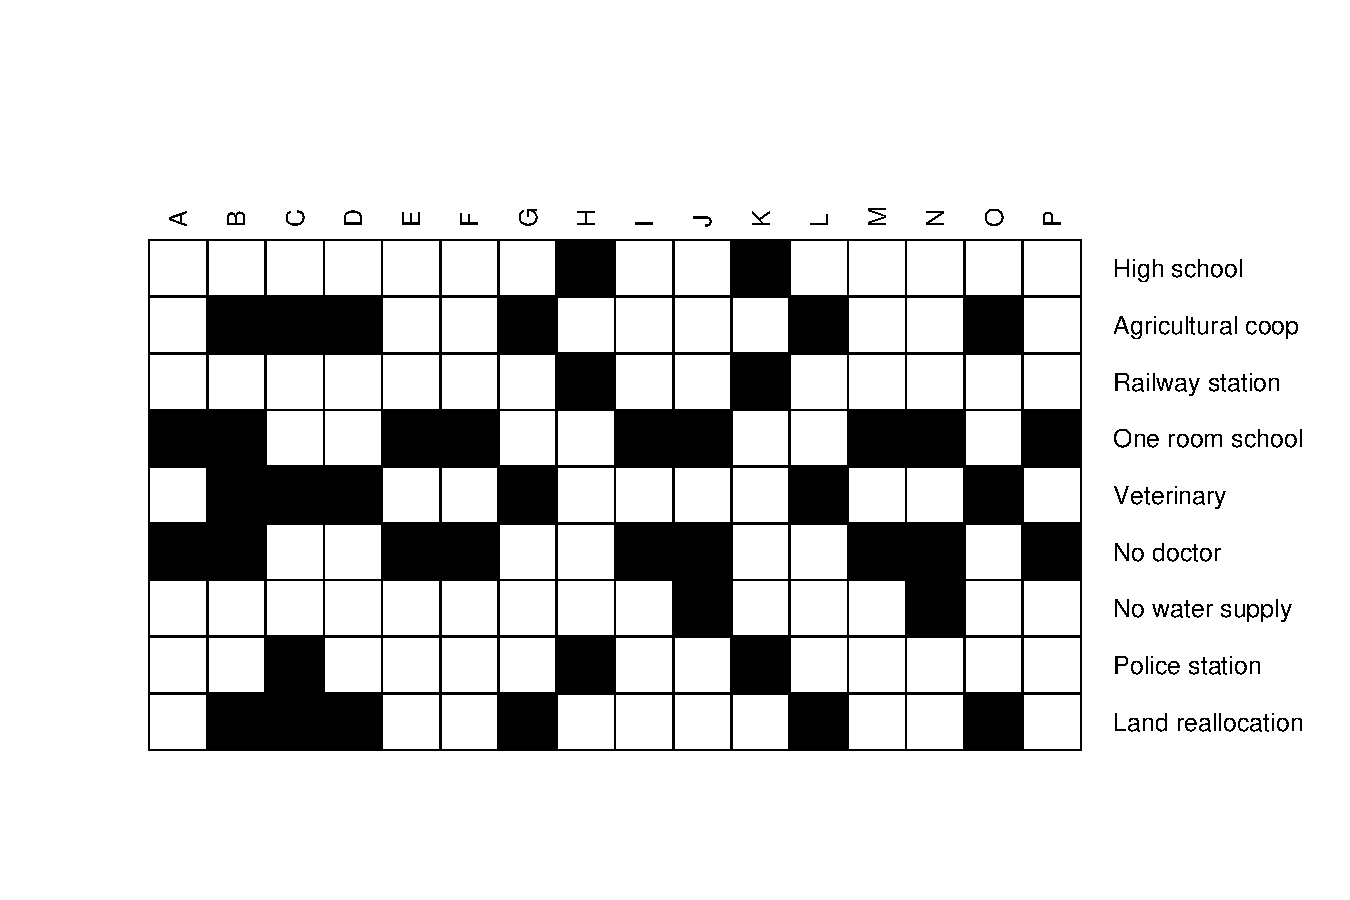
\includegraphics[width=12cm, trim=0 40 0 30]{seriation-binary1} \\
    (a)    

    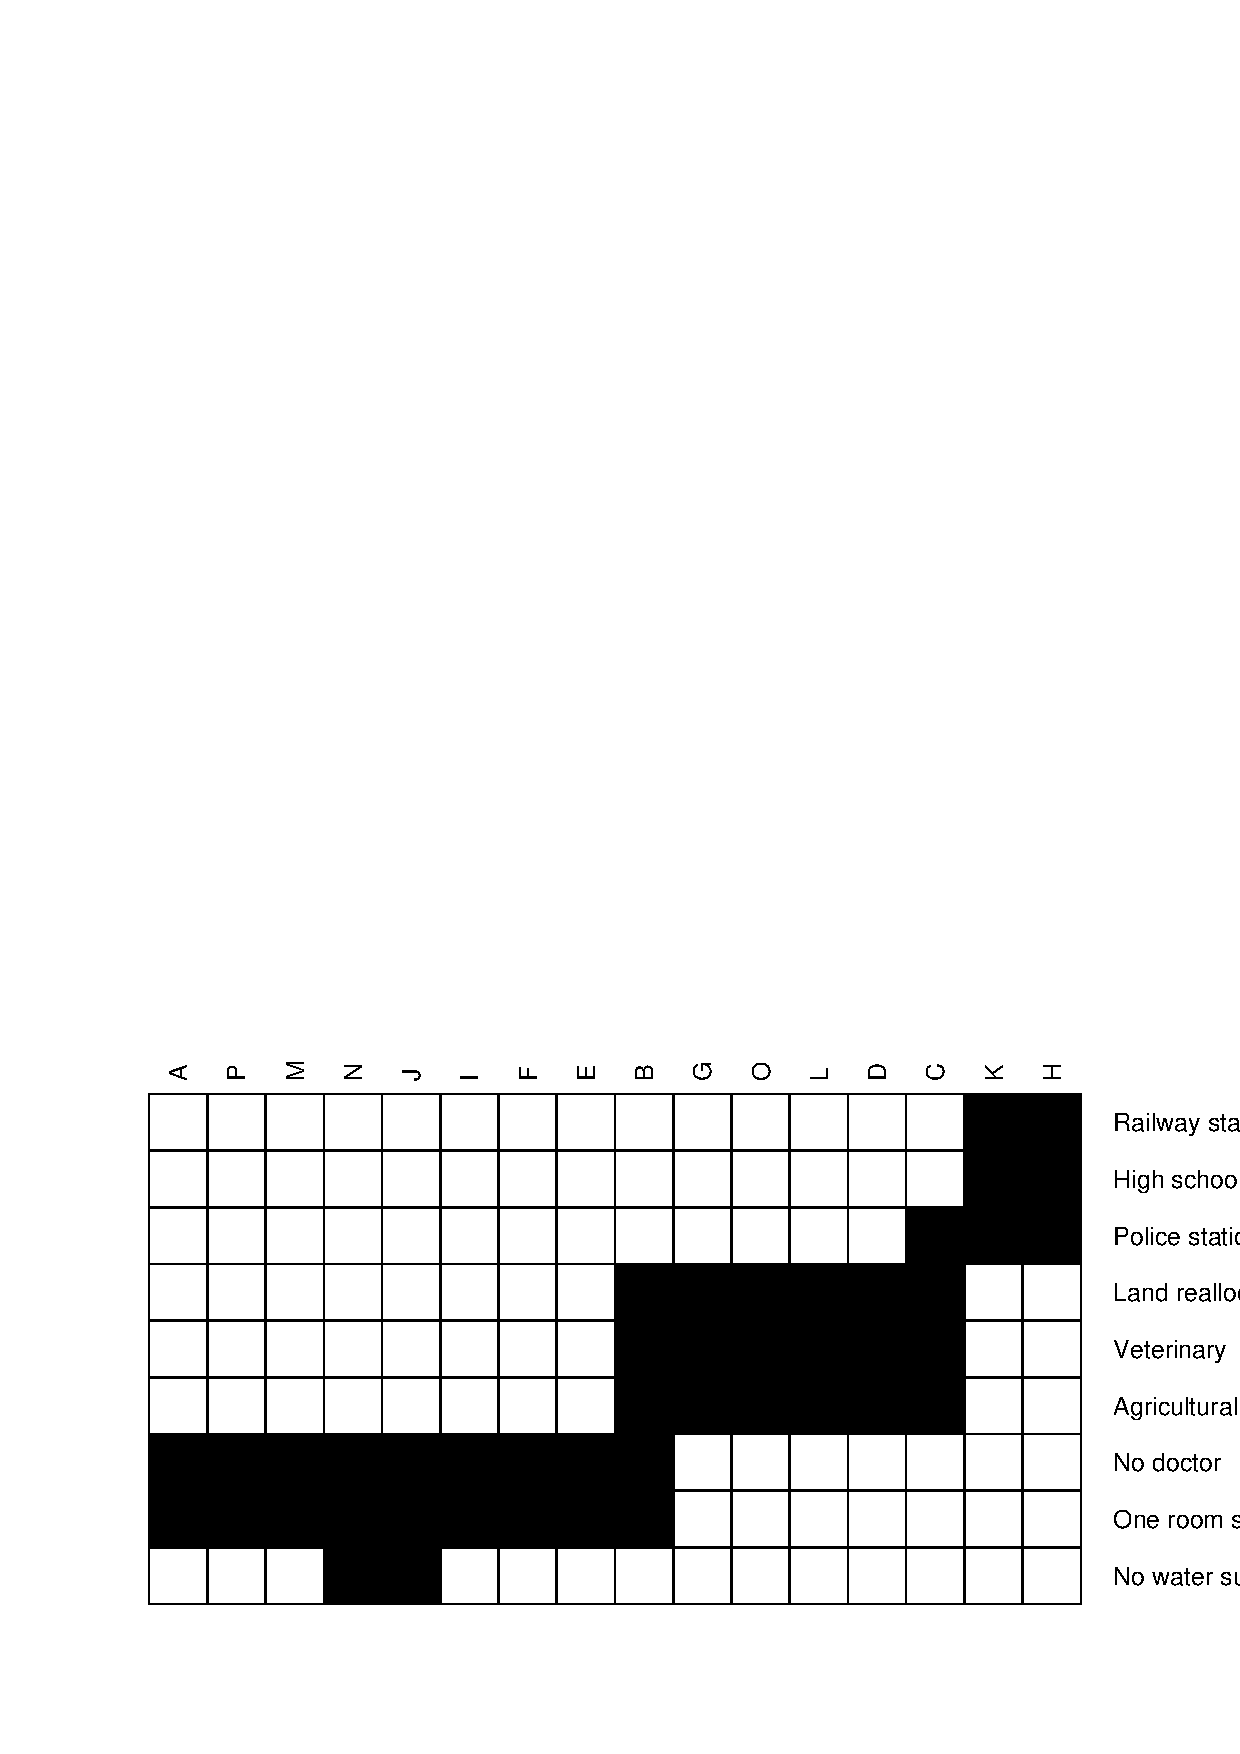
\includegraphics[width=12cm, trim=0 40 0 30]{seriation-binary2} \\
    (b)   

    \caption{The townships data set in original order (a) and 
    reordered using BEA (b).}
    \label{fig:binary}
\end{figure}


\begin{Schunk}
\begin{Sinput}
> rbind(original = criterion(Townships), reordered = criterion(Townships, 
+     order))
\end{Sinput}
\begin{Soutput}
          ME Moore_stress Neumann_stress
original  19          464            260
reordered 65          212             82
\end{Soutput}
\end{Schunk}

BEA tries to maximize the measure of effectiveness which is
much higher in the reordered matrix (in fact, 65 is the maximum for 
the data set). Also the two types of stress are improved
significantly.

\subsection{Dissimilarity plot}

Assessing the quality of an obtained cluster solution has been a
research topic since the invention of cluster analysis. This is
especially important since all popular cluster algorithms produce a
clustering even for data without a ``cluster'' structure.

%A method to judge the quality of a cluster solution is by inspecting a
%visualization. For hierarchical clustering
%dendrogramms~\cite{seriation:Hartigan:1967} are available which show the
%hierarchical structure of the clustering as a binary tree and cluster quality 
%can be judged by looking at the dissimilarities between objects in a cluster
%and objects in other clusters. However, such a visualization is
%only possible for heirarchical/nested clusterings. 
%
%\marginpar{Cite Pison et al 1999 and Kaufmann and Rousseeuw}
%For the an arbitrary partitional clustering, the original objects can
%be displayed in a 2 dimensional scatter plot
%after using dimensionality reduction (e.g., PCA, MDS).
%Objects belonging to the same cluster can be marked and thus, if the
%dimensionality reduction preserves a large proportion of the
%variavility in the original data, the separation between clusters can be
%visually judged.
%
%Silhouettes

Matrix shading is an old technique to visualize clusterings by displaying the
rearranged matrices~\citep[see,
e.g.,][]{seriation:Sneath:1973,seriation:Ling:1973,seriation:Gale:1984}.
Initially matrix shading was used in connection with hierarchical clustering,
where the order of the dendrograms leaf nodes was used to arrange the matrix.
However, with some extensions, matrix shading can be also used with any
partitional clustering method. 

\cite{seriation:Strehl:2003} suggest a matrix shading visualization called
\emph{CLUSION} where the dissimilarity matrix is arranged such that all objects
pertaining to a single cluster appear in consecutive order in the matrix. The
authors call this \emph{coarse seriation}. The result of a ``good'' clustering
should be a matrix with low dissimilarity values forming blocks around the main
diagonal.  However, using coarse seriation, the order of the clusters has to be
predefined and the objects within each cluster are unordered.

Dissimilarity plots as produce by \func{dissplot} aims a reflecting
global structure between clusters as well as the micro structure within
clusters. To achieve this, we arrange the clusters as well as the
objects within each cluster using seriation techniques.  To arrange
clusters, an inter-cluster dissimilarity matrix is calculated using the
average between cluster dissimilarities. \func{seriate} is used on this
inter-cluster dissimilarity matrix to arrange the clusters relative to
each other resulting in on average more similar clusters to appear
closer together.  Within each cluster, \func{seriate} is used again on
the sub-matrix of the dissimilarity matrix concerning only the objects
in the cluster.

For the example, we use again Euclidean distance between the objects in the
iris data set.

\begin{Schunk}
\begin{Sinput}
> data("iris")
> iris <- iris[sample(seq_len(nrow(iris))), ]
> d <- dist(as.matrix(iris[-5]), method = "euclidean")
\end{Sinput}
\end{Schunk}

First, we use \func{dissplot} without a clustering. We set \code{method}
to \code{NA} to prevent reordering and display the original matrix. Then
we omit the method argument which results in using the default seriation
technique from \func{seriate.dist} which is a TSP heuristic. Since we did
not provide a clustering, the whole matrix is reordered in one piece.
The result in shown in Figure~\ref{fig:dissplot1}.
From Figure~\ref{fig:dissplot1}(b) it seems that there is a clear structure in
the data which suggests a two cluster solution.

\begin{Schunk}
\begin{Sinput}
> dissplot(d, method = NA)
\end{Sinput}
\end{Schunk}

\begin{Schunk}
\begin{Sinput}
> dissplot(d, options = list(main = "Seriation (TSP)"))
\end{Sinput}
\end{Schunk}



\begin{figure}
    \begin{minipage}[b]{.48\linewidth}
    \centering
    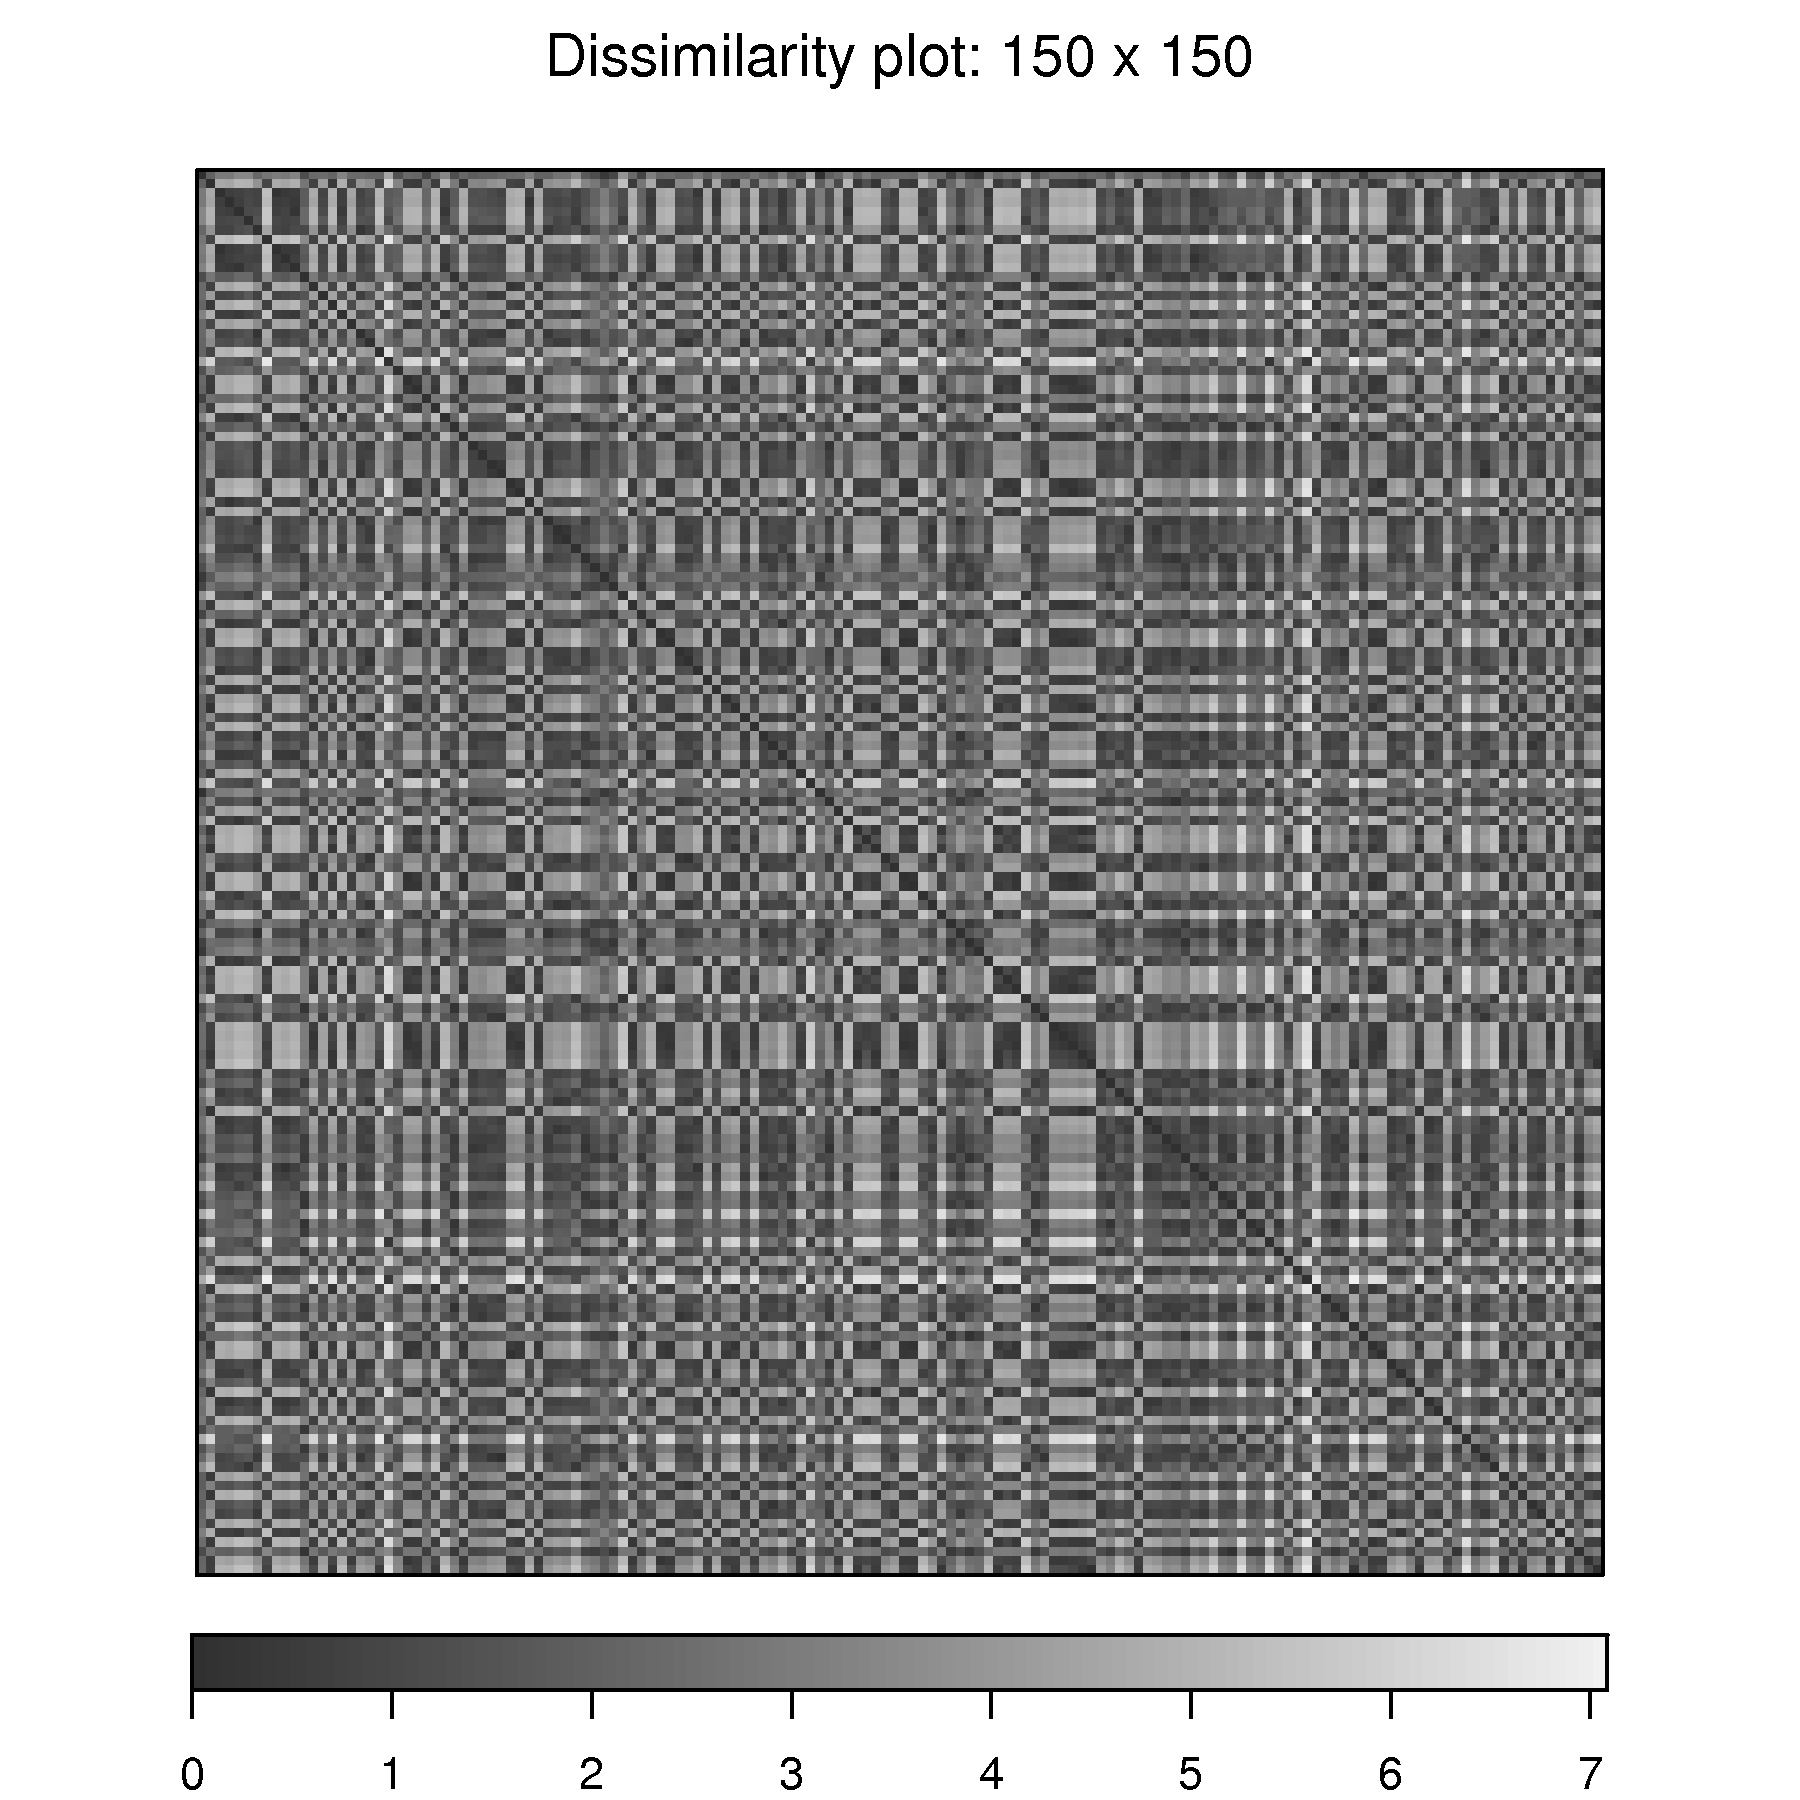
\includegraphics[width=\linewidth]{seriation-dissplot1} \\
    (a)    
    \end{minipage}
    \begin{minipage}[b]{.48\linewidth}
    \centering
    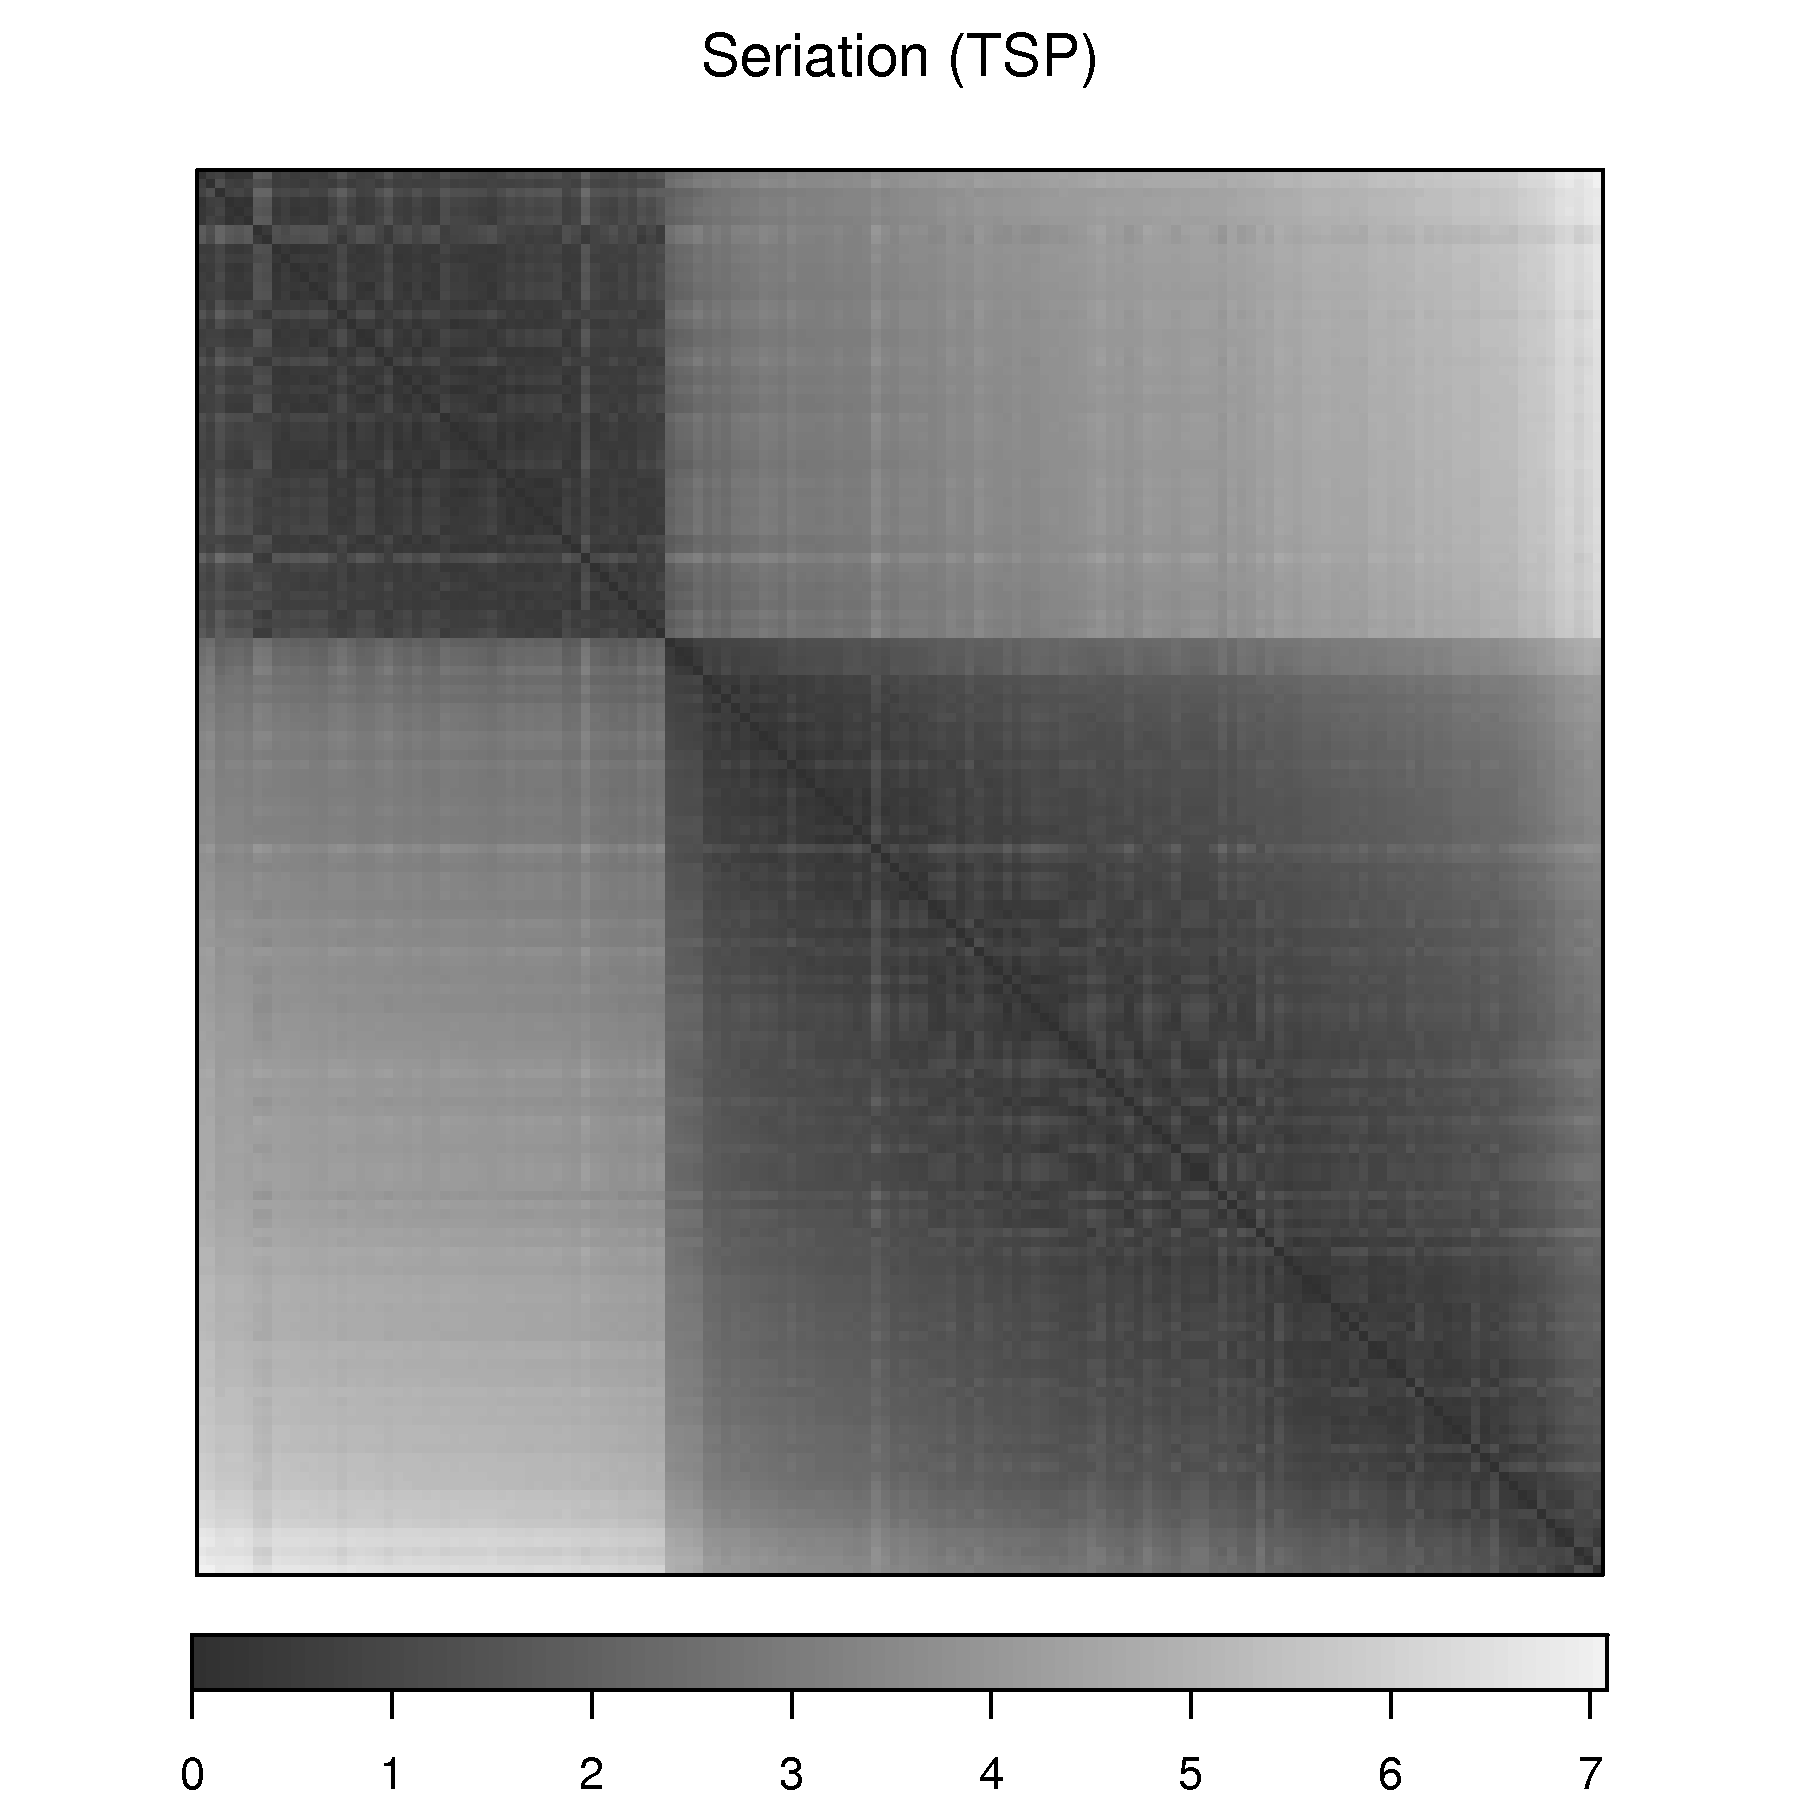
\includegraphics[width=\linewidth]{seriation-dissplot2} \\
    (b)   
    \end{minipage}
    \caption{Two dissimilarity plots. 
    (a) the original dissimilarity matrix and 
    (b) the seriated dissimilarity matrix.}
    \label{fig:dissplot1}
\end{figure}

Next, we create a cluster solution using $k$-means. Although we know
that the data set should contain $3$ groups representing the three species
of iris, we let $k$-means produce a $10$ cluster solution to study how such a 
misspecification can be spotted using \func{dissplot}.


\begin{Schunk}
\begin{Sinput}
> l <- kmeans(d, 10)$cluster
\end{Sinput}
\end{Schunk}

We create a standard dissimilarity plot by providing the cluster
solution as a vector of labels. The function rearranges the matrix and
plots the result. Since rearrangement can be a time consuming procedure for
large matrices, the rearranged matrix and all
information needed for plotting is returned as the result. 

\begin{Schunk}
\begin{Sinput}
> res <- dissplot(d, labels = l, options = list(main = "Seriation - standard"))
\end{Sinput}
\end{Schunk}

\begin{figure}
    \centering
    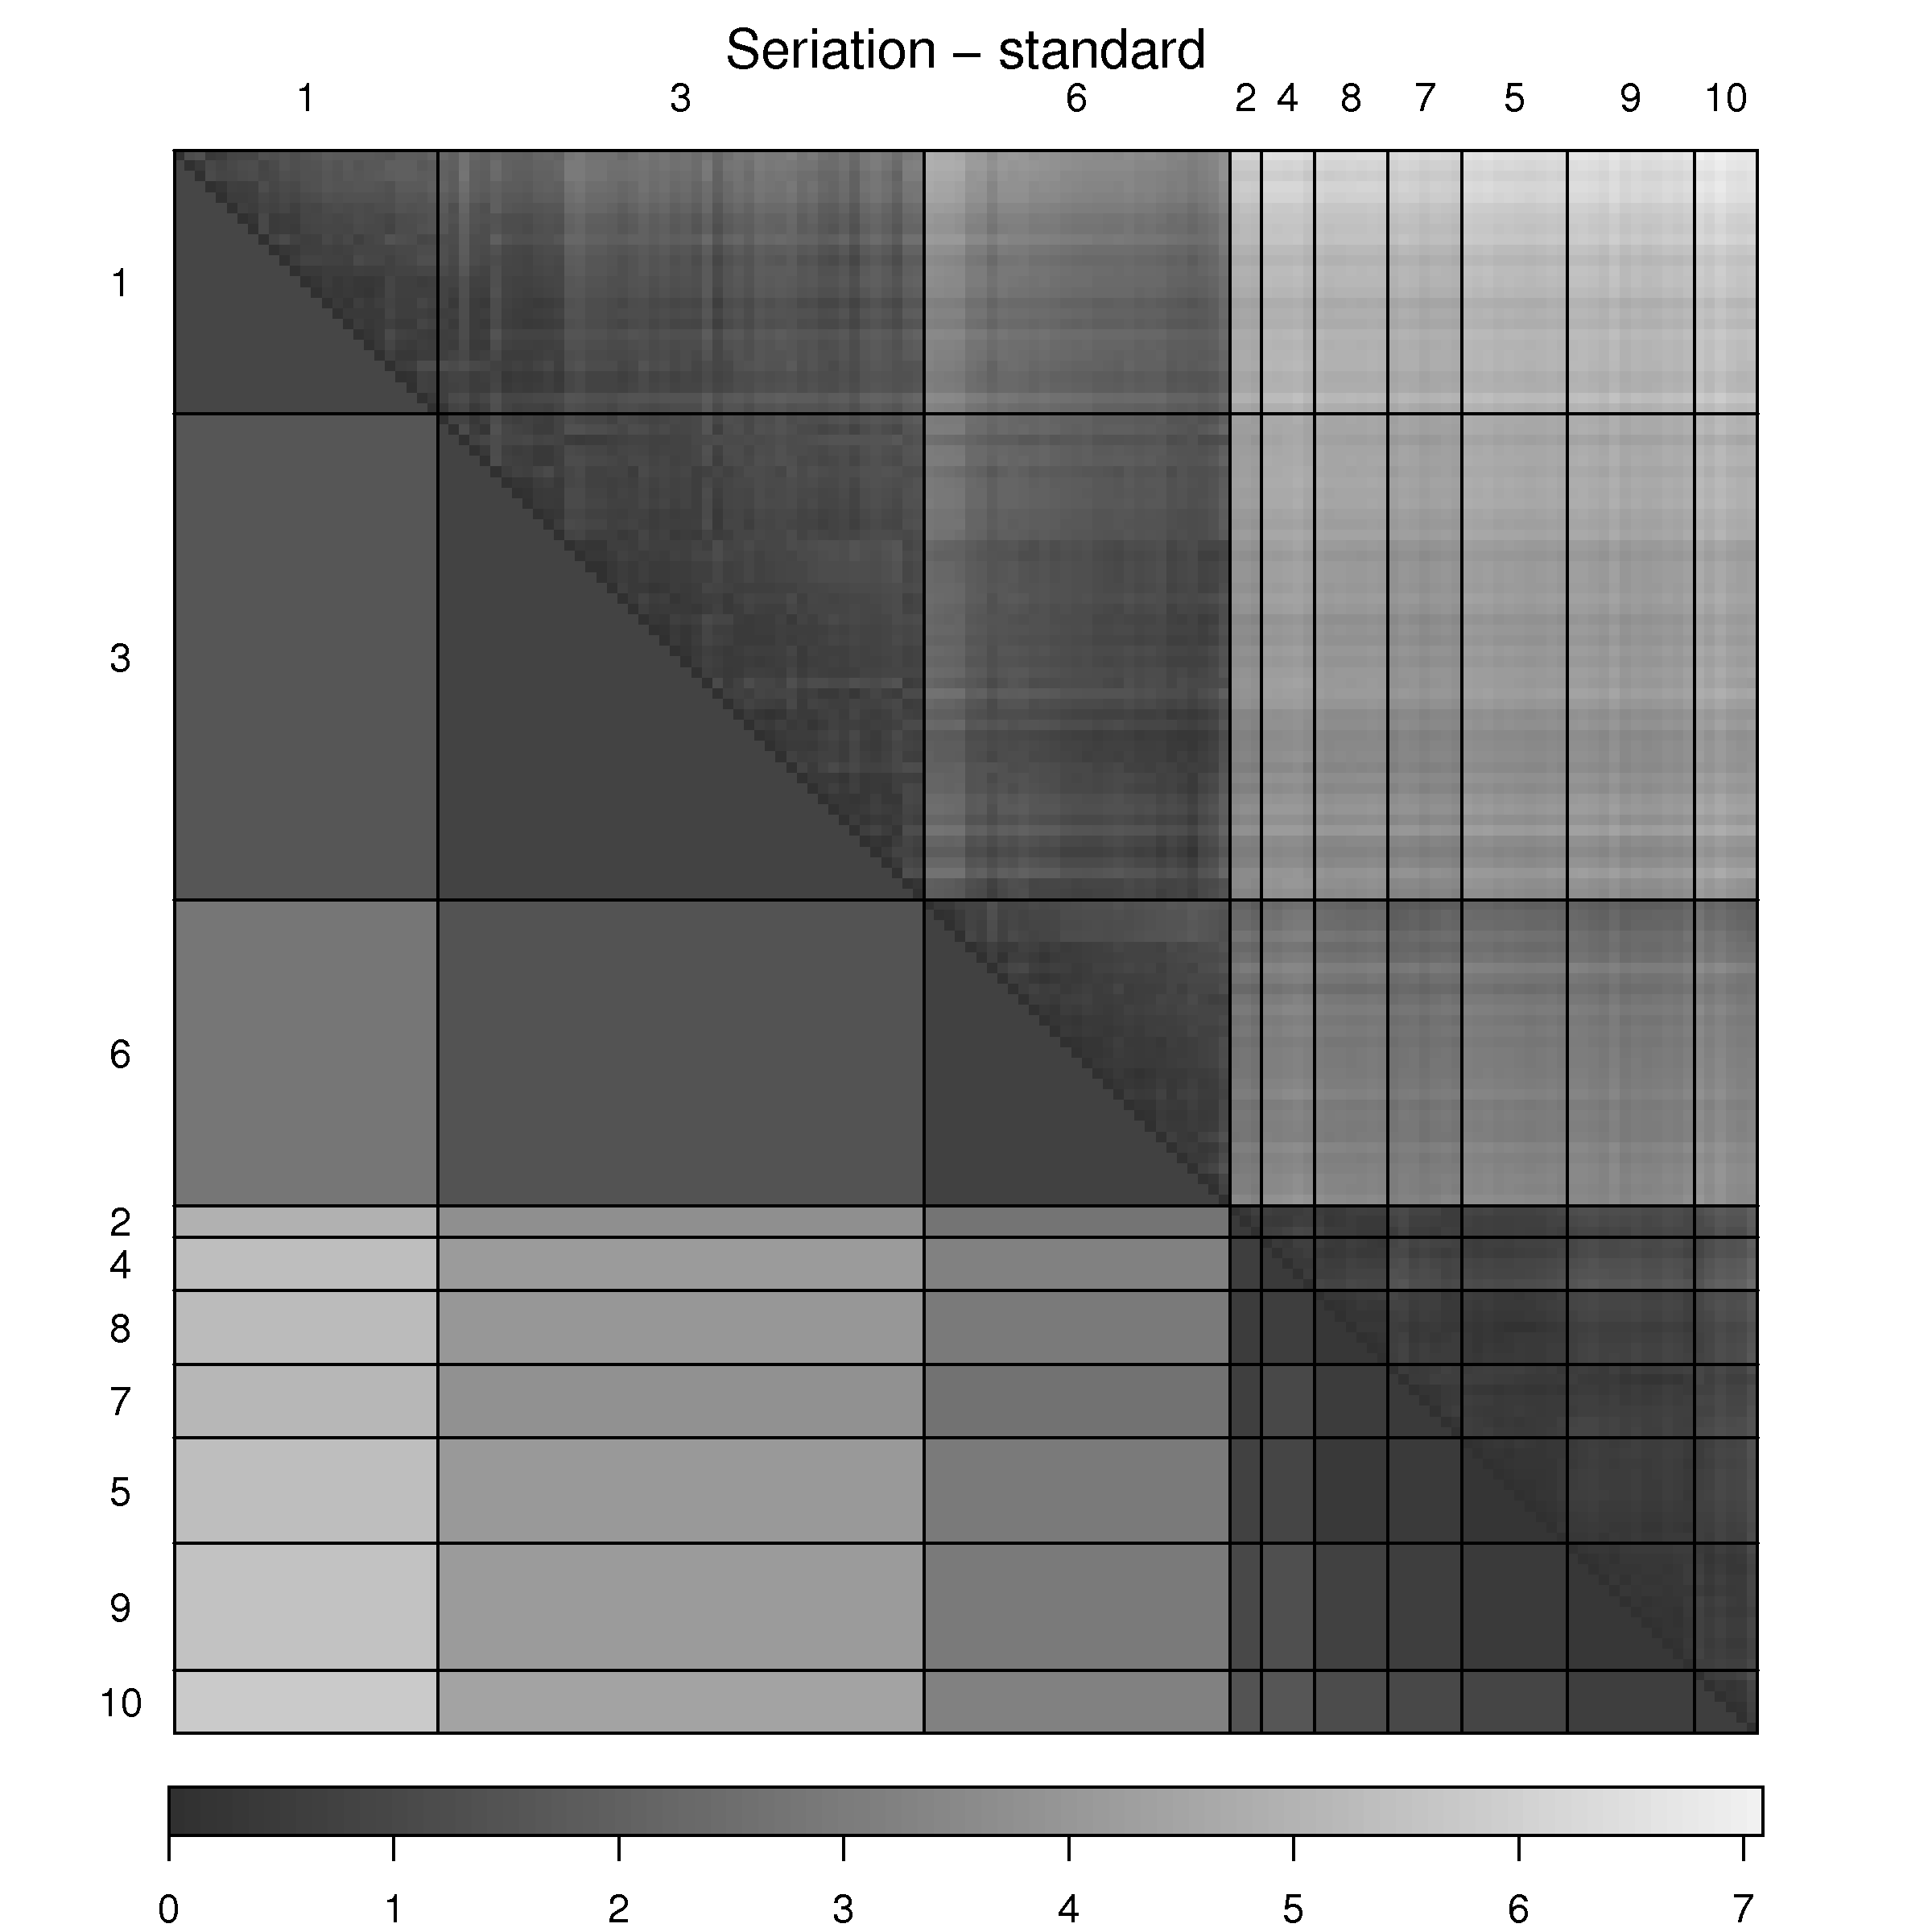
\includegraphics[width=10cm]{seriation-dissplot3}\\
    (a)
    
    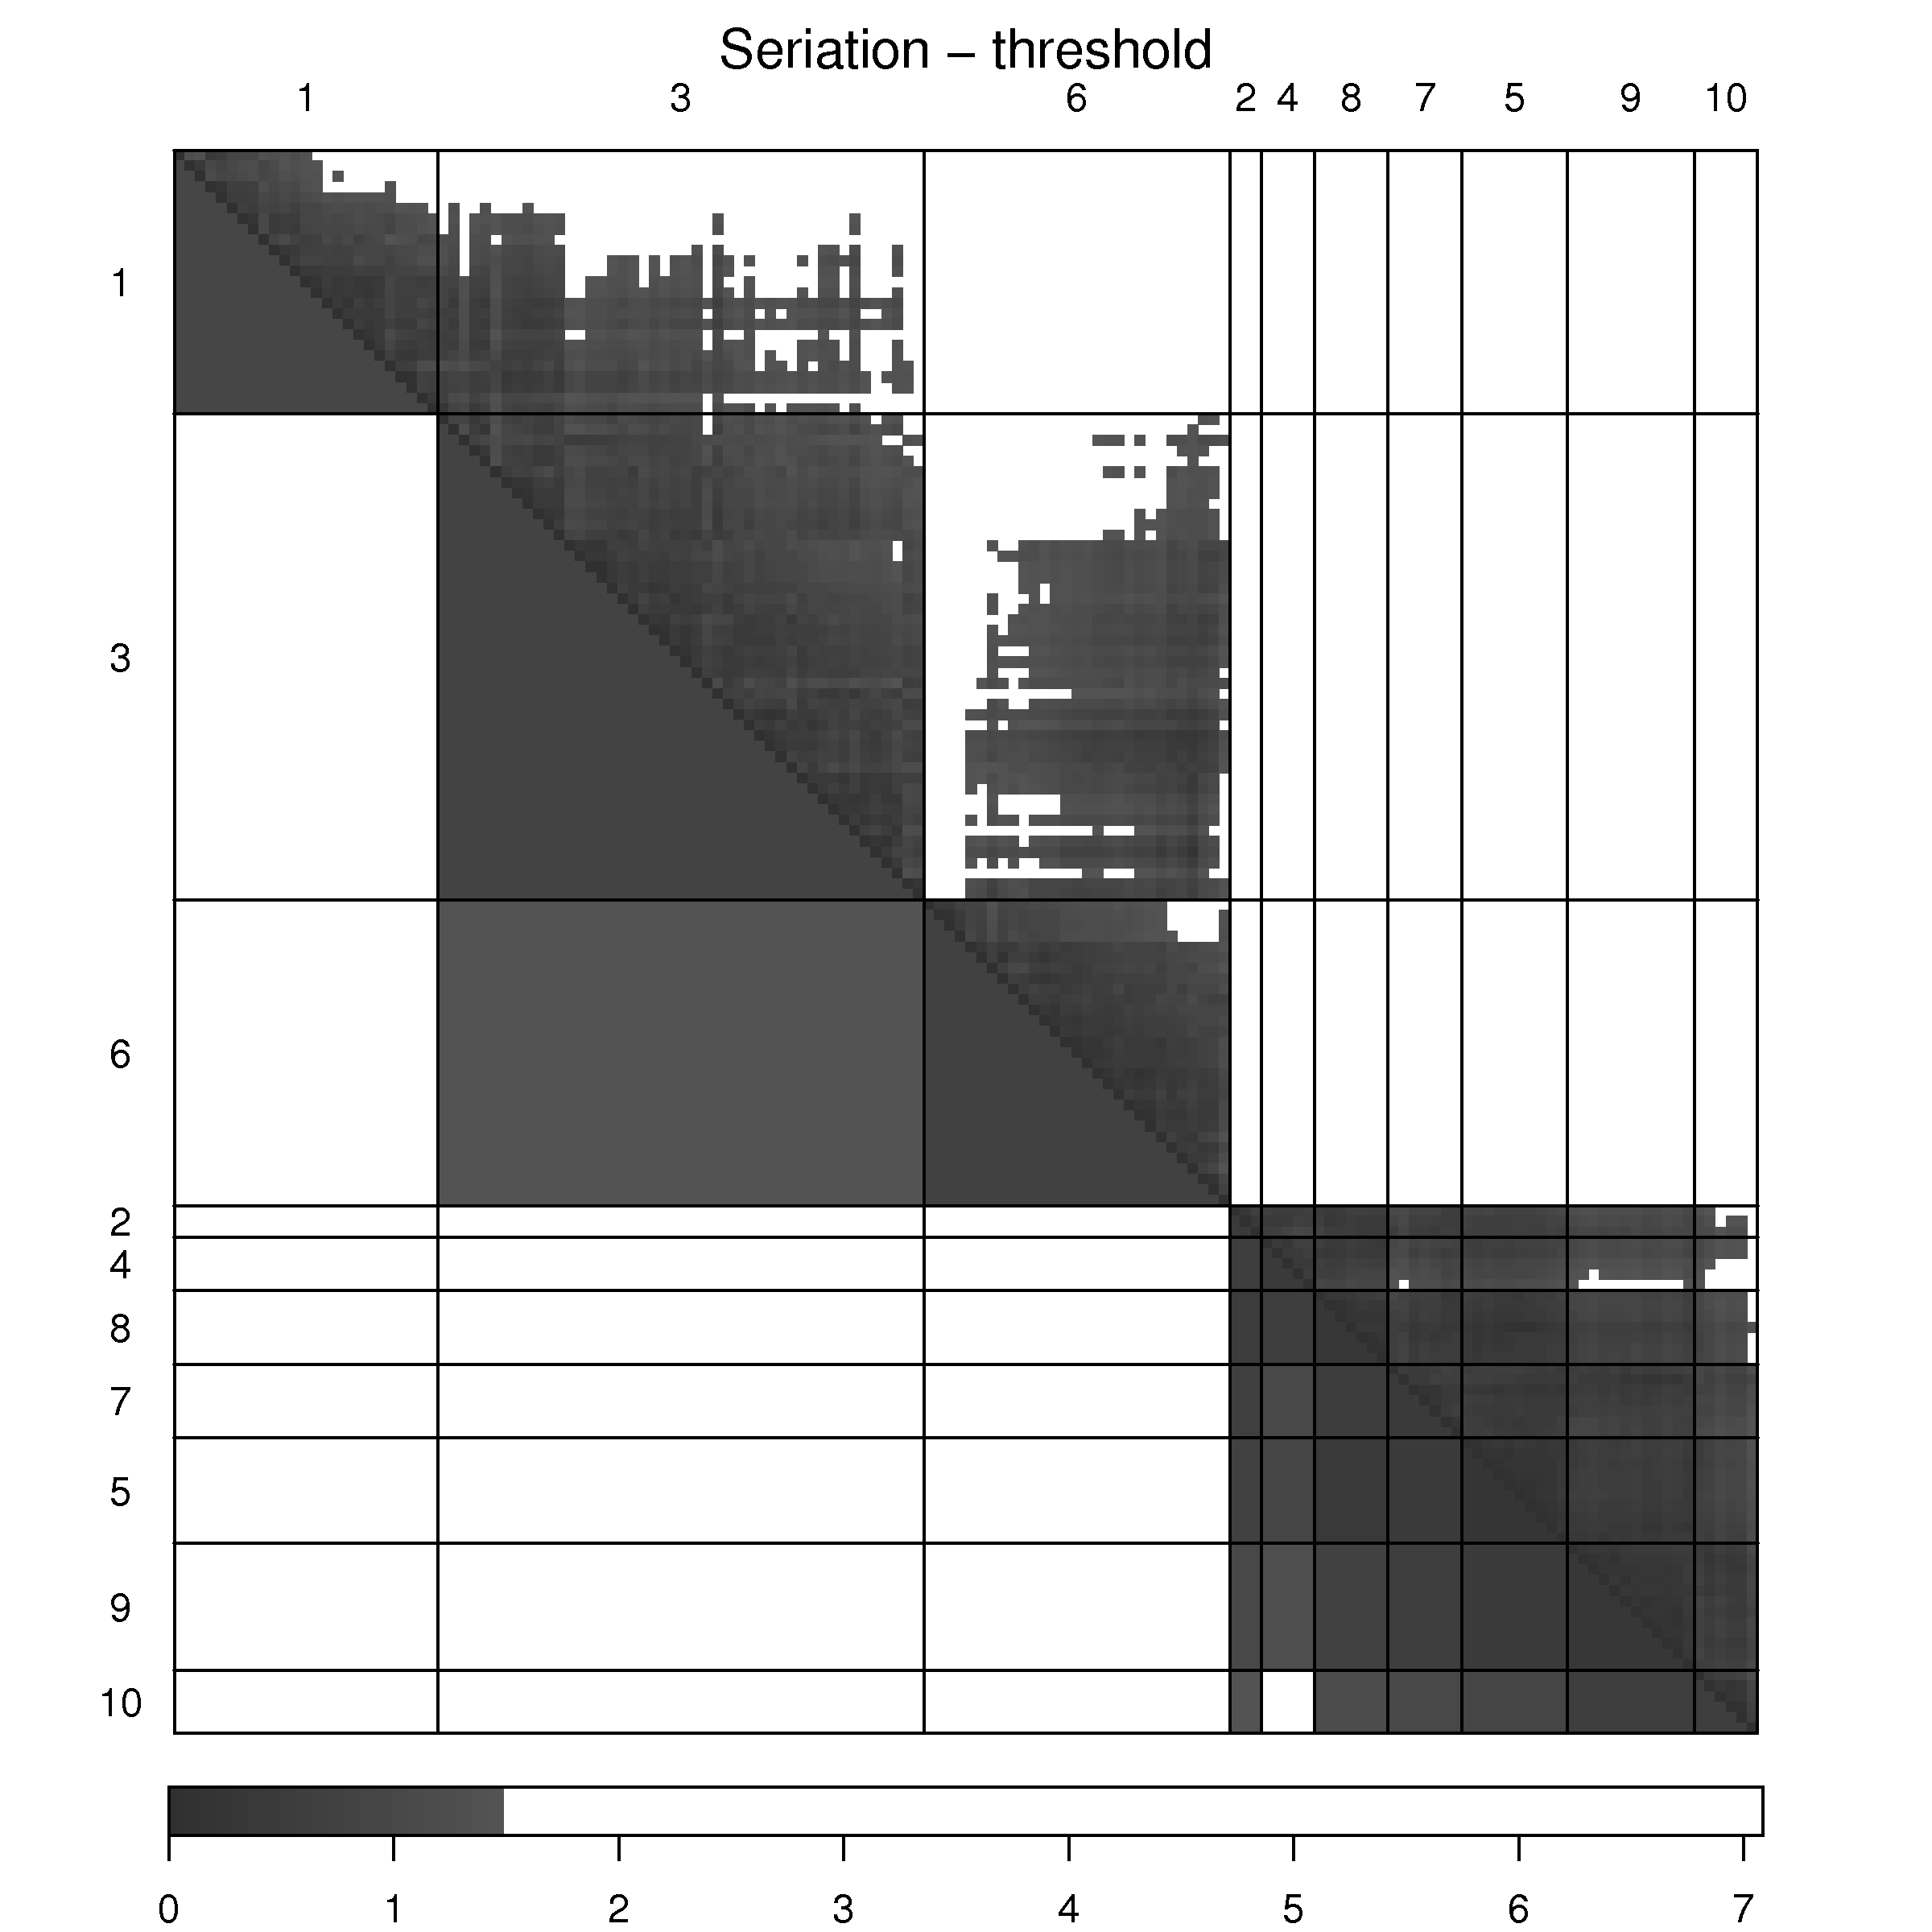
\includegraphics[width=10cm]{seriation-dissplot4}\\
    (b)
    \caption{Dissimilarity plot for $k$-means solution with 10 clusters. 
    (a) standard plot and (b) plot with threshold.}
    \label{fig:dissplot3}
\end{figure}

\begin{Schunk}
\begin{Sinput}
> res
\end{Sinput}
\begin{Soutput}
object of class ‘cluster_dissimilarity_matrix’ 
matrix dimensions: x 
dissimilarity measure: ‘euclidean’ 
number of clusters k: 10 

cluster description
   position label size avg_dissimilarity avg_silhouette_width
1         1     1   25            0.9794              0.34635
2         2     3   46            0.7754              0.31231
3         3     6   29            0.3124              0.43920
4         4     2    3            0.8411              0.10950
5         5     4    5            0.4487              0.14042
6         6     8    7            0.2396              0.18984
7         7     7    7            0.4663             -0.08724
8         8     5   10            0.4939              0.34195
9         9     9   12            0.2942              0.36239
10       10    10    6            0.5795              0.03654

used seriation methods
inter-cluster: ‘ARSA’ 
intra-cluster: ‘ARSA’ 
\end{Soutput}
\end{Schunk}

The resulting plot is shown in Figure~\ref{fig:dissplot3}(a).  The
inter-cluster dissimilarities are shown as gray blocks and the average object
dissimilarity within each cluster as gray triangles below the main diagonal of
the matrix. Since the clusters are arranged such that more similar clusters
are closer together, it is easy to see in Figure~\ref{fig:dissplot3}(a)
that clusters 1, 3 and 6 as well as clusters 2, 4, 8, 5, 7, 9 and 10 
are very similar and form two blocks. 
This suggests again that a two cluster solution would
be reasonable.

Since slight variations of gray values are hard to distinguish,
we plot the matrix again (using \func{plot} on the result above) and
use a threshold on the dissimilarity to suppress high dissimilarity
values in the plot. 

\begin{Schunk}
\begin{Sinput}
> plot(res, options = list(main = "Seriation - threshold", 
+     threshold = 1.5))
\end{Sinput}
\end{Schunk}

In the resulting plot in Figure~\ref{fig:dissplot3}(b), we see that the
block containing 2, 4, 8, 5, 7, 9 and 10 is very well defined and
cleanly separated from the other block. This suggests that these clusters
should form together a cluster in a solution with less clusters.
The other block is less well defined. There is considerable overlap between
clusters 3 and 6, but also cluster 1 and 3 share similar objects.

Using the information stored in the result of \func{dissplot} and
the class information available for the iris data set, we can analyze
the cluster solution and the interpretations of the dissimilarity plot.

\begin{Schunk}
\begin{Sinput}
> table(iris[res$order, 5], res$label)[, res$cluster_order]
\end{Sinput}
\begin{Soutput}
              1  3  6 2 4 8 7  5  9 10
  setosa      0  0  0 3 5 7 7 10 12  6
  versicolor  0 22 28 0 0 0 0  0  0  0
  virginica  25 24  1 0 0 0 0  0  0  0
\end{Soutput}
\end{Schunk}

As the plot in Figure~\ref{fig:dissplot3} indicated, the clusters 2, 4, 8, 5,
7, 9 and 10 should be a single cluster containing only flowers of the species
Iris setosa. The clusters 1, 3 and 6 are more problematic since they contain a
mixture of Iris versicolor and virginica.

\section{Conclusion}
\label{sec:conclusion}

In this paper we presented the infrastructure provided by the
package~\pkg{seriation}. The infrastructure contains the necessary data
structures to store the linear order for one-, two- and $k$-mode data.  It also
provides a wide array of seriation methods for different input data, e.g.,
dissimilarities, binary and general data matrices focusing on combinatorial
optimization.

Based on seriation, several visualization techniques are provided by
\pkg{seriation}.  In particular, the optimally reordered heat map, the
Bertin plot and the dissimilarity plot present clear improvements over
standard plots.

Future work on \pkg{seriation} will focus on adding further seriation
methods, such as for example methods for block seriation which aim at
finding simultaneous partitions of rows and columns in a data
matrix~\citep[see, e.g.,][]{seriation:Marcotorchino:1987}.


\section*{Acknowledgments}
The authors would like to thank Michael Brusco, Hans-Friedrich K{\"o}hn and
Stephanie Stahl for their seriation code, and Fionn Murtagh for his BEA
implementation.  

%
{\small
\bibliographystyle{abbrvnat}
\bibliography{seriation}
}
%
\end{document}

